\documentclass{book}
\usepackage[a4paper,top=2.5cm,bottom=2.5cm,left=2.5cm,right=2.5cm]{geometry}
\usepackage{makeidx}
\usepackage{natbib}
\usepackage{graphicx}
\usepackage{multicol}
\usepackage{float}
\usepackage{listings}
\usepackage{color}
\usepackage{ifthen}
\usepackage[table]{xcolor}
\usepackage{textcomp}
\usepackage{alltt}
\usepackage{ifpdf}
\ifpdf
\usepackage[pdftex,
            pagebackref=true,
            colorlinks=true,
            linkcolor=blue,
            unicode
           ]{hyperref}
\else
\usepackage[ps2pdf,
            pagebackref=true,
            colorlinks=true,
            linkcolor=blue,
            unicode
           ]{hyperref}
\usepackage{pspicture}
\fi
\usepackage[utf8]{inputenc}
\usepackage{mathptmx}
\usepackage[scaled=.90]{helvet}
\usepackage{courier}
\usepackage{sectsty}
\usepackage{amssymb}
\usepackage[titles]{tocloft}
\usepackage{doxygen}
\lstset{language=C++,inputencoding=utf8,basicstyle=\footnotesize,breaklines=true,breakatwhitespace=true,tabsize=8,numbers=left }
\makeindex
\setcounter{tocdepth}{3}
\renewcommand{\footrulewidth}{0.4pt}
\renewcommand{\familydefault}{\sfdefault}
\hfuzz=15pt
\setlength{\emergencystretch}{15pt}
\hbadness=750
\tolerance=750
\begin{document}
\hypersetup{pageanchor=false,citecolor=blue}
\begin{titlepage}
\vspace*{7cm}
\begin{center}
{\Large libcollider }\\
\vspace*{1cm}
{\large Generated by Doxygen 1.8.3.1-20130209}\\
\vspace*{0.5cm}
{\small Sat Jun 8 2013 10:53:11}\\
\end{center}
\end{titlepage}
\clearemptydoublepage
\pagenumbering{roman}
\tableofcontents
\clearemptydoublepage
\pagenumbering{arabic}
\hypersetup{pageanchor=true,citecolor=blue}
\chapter{Hierarchical Index}
\section{Class Hierarchy}
This inheritance list is sorted roughly, but not completely, alphabetically\-:\begin{DoxyCompactList}
\item \contentsline{section}{sc\-:\-:Buffer}{\pageref{classsc_1_1Buffer}}{}
\item \contentsline{section}{sc\-:\-:Bus}{\pageref{classsc_1_1Bus}}{}
\item \contentsline{section}{sc\-:\-:Node}{\pageref{classsc_1_1Node}}{}
\begin{DoxyCompactList}
\item \contentsline{section}{sc\-:\-:Group}{\pageref{classsc_1_1Group}}{}
\begin{DoxyCompactList}
\item \contentsline{section}{sc\-:\-:Root\-Node}{\pageref{classsc_1_1RootNode}}{}
\end{DoxyCompactList}
\item \contentsline{section}{sc\-:\-:Synth}{\pageref{classsc_1_1Synth}}{}
\end{DoxyCompactList}
\item \contentsline{section}{sc\-:\-:S\-C\-Server}{\pageref{classsc_1_1SCServer}}{}
\item \contentsline{section}{sc\-:\-:Sound}{\pageref{classsc_1_1Sound}}{}
\end{DoxyCompactList}

\chapter{Class Index}
\section{Class List}
Here are the classes, structs, unions and interfaces with brief descriptions\-:\begin{DoxyCompactList}
\item\contentsline{section}{\hyperlink{classColliderPlusPlus_1_1Buffer}{Collider\-Plus\-Plus\-::\-Buffer} \\*This class represents a client-\/side version of a server buffer }{\pageref{classColliderPlusPlus_1_1Buffer}}{}
\item\contentsline{section}{\hyperlink{classColliderPlusPlus_1_1Bus}{Collider\-Plus\-Plus\-::\-Bus} }{\pageref{classColliderPlusPlus_1_1Bus}}{}
\item\contentsline{section}{\hyperlink{classColliderPlusPlus_1_1Client__Server}{Collider\-Plus\-Plus\-::\-Client\-\_\-\-Server} \\*This class represents a client-\/side version of scsynth, the Super\-Collider audio server }{\pageref{classColliderPlusPlus_1_1Client__Server}}{}
\item\contentsline{section}{\hyperlink{classColliderPlusPlus_1_1Group}{Collider\-Plus\-Plus\-::\-Group} \\*This class represents a client-\/side version of a server group }{\pageref{classColliderPlusPlus_1_1Group}}{}
\item\contentsline{section}{\hyperlink{classColliderPlusPlus_1_1Node}{Collider\-Plus\-Plus\-::\-Node} \\*This class represents a client-\/side version of a server node (\hyperlink{classColliderPlusPlus_1_1Synth}{Synth} or \hyperlink{classColliderPlusPlus_1_1Group}{Group}) }{\pageref{classColliderPlusPlus_1_1Node}}{}
\item\contentsline{section}{\hyperlink{classColliderPlusPlus_1_1RootNode}{Collider\-Plus\-Plus\-::\-Root\-Node} \\*This class represents a client-\/side version of a server root node }{\pageref{classColliderPlusPlus_1_1RootNode}}{}
\item\contentsline{section}{\hyperlink{classColliderPlusPlus_1_1Sound}{Collider\-Plus\-Plus\-::\-Sound} \\*This class represents a user manipulable Soundfile Player, essentially mirroring the O\-A\-S class of the same name by Shreenidhi Chowkwale  \href{https://github.com/CalVR/Open-Audio-Server/blob/master/client/src/Sound.h}{\tt https\-://github.\-com/\-Cal\-V\-R/\-Open-\/\-Audio-\/\-Server/blob/master/client/src/\-Sound.\-h} }{\pageref{classColliderPlusPlus_1_1Sound}}{}
\item\contentsline{section}{\hyperlink{classColliderPlusPlus_1_1Synth}{Collider\-Plus\-Plus\-::\-Synth} \\*This class represents a client-\/side version of a server synth }{\pageref{classColliderPlusPlus_1_1Synth}}{}
\end{DoxyCompactList}

\chapter{File Index}
\section{File List}
Here is a list of all documented files with brief descriptions\-:\begin{DoxyCompactList}
\item\contentsline{section}{include/\hyperlink{Buffer_8hpp}{Buffer.\-hpp} \\*Header file for \hyperlink{Buffer_8hpp}{Buffer.\-hpp} }{\pageref{Buffer_8hpp}}{}
\item\contentsline{section}{include/\hyperlink{Bus_8hpp}{Bus.\-hpp} \\*Header file for \hyperlink{Bus_8hpp}{Bus.\-hpp} }{\pageref{Bus_8hpp}}{}
\item\contentsline{section}{include/{\bfseries libcollider.\-hpp} }{\pageref{libcollider_8hpp}}{}
\item\contentsline{section}{include/\hyperlink{Node_8hpp}{Node.\-hpp} \\*Header file for \hyperlink{Node_8hpp}{Node.\-hpp} }{\pageref{Node_8hpp}}{}
\item\contentsline{section}{include/\hyperlink{SCServer_8hpp}{S\-C\-Server.\-hpp} \\*Header file for \hyperlink{SCServer_8hpp}{S\-C\-Server.\-hpp} }{\pageref{SCServer_8hpp}}{}
\item\contentsline{section}{include/\hyperlink{Sound_8hpp}{Sound.\-hpp} \\*Header file for \hyperlink{Sound_8hpp}{Sound.\-hpp} }{\pageref{Sound_8hpp}}{}
\end{DoxyCompactList}

\chapter{Class Documentation}
\hypertarget{classsc_1_1Buffer}{\section{sc\-:\-:Buffer Class Reference}
\label{classsc_1_1Buffer}\index{sc\-::\-Buffer@{sc\-::\-Buffer}}
}


This class represents a client-\/side version of a server buffer.  




{\ttfamily \#include $<$Buffer.\-hpp$>$}

\subsection*{Public Member Functions}
\begin{DoxyCompactItemize}
\item 
\hyperlink{classsc_1_1Buffer_aa461325a96603e78a79561e90ce5f394}{Buffer} (\hyperlink{classsc_1_1SCServer}{S\-C\-Server} $\ast$other, int buf\-Num)
\item 
\hypertarget{classsc_1_1Buffer_ab9ef17039f271262d3c3dbc979cdc85d}{\hyperlink{classsc_1_1Buffer_ab9ef17039f271262d3c3dbc979cdc85d}{$\sim$\-Buffer} ()}\label{classsc_1_1Buffer_ab9ef17039f271262d3c3dbc979cdc85d}

\begin{DoxyCompactList}\small\item\em Destructor. \end{DoxyCompactList}\item 
int \hyperlink{classsc_1_1Buffer_af777b92a6ba7b4330fb9958141282cc9}{get\-Buf\-Num} () const 
\item 
int \hyperlink{classsc_1_1Buffer_a591c50bcaae889d763ff28688febeb71}{get\-Frame\-Num} () const 
\item 
int \hyperlink{classsc_1_1Buffer_a57f2455044a2303a1fba1d17e2a7470c}{get\-Chan\-Num} () const 
\item 
int \hyperlink{classsc_1_1Buffer_a15c75bed82addc4ec16b74e98e5ee770}{get\-Samp\-Rate} () const 
\item 
bool \hyperlink{classsc_1_1Buffer_aa3002f528e1eda702d29626004069491}{get\-Manually\-Freed} () const 
\item 
void \hyperlink{classsc_1_1Buffer_a444402b37e84ca30c529df66749c897d}{set\-Buf\-Num} (int bn)
\item 
void \hyperlink{classsc_1_1Buffer_a4ed9a45c0ac7c1b4d7cda850153bfb4a}{set\-Num\-Frames} (unsigned long nf)
\item 
void \hyperlink{classsc_1_1Buffer_afd3831ddbad9748d31dd6260ba6392fc}{set\-Num\-Chans} (int nc)
\item 
void \hyperlink{classsc_1_1Buffer_a9ba693d9d86afaccce4d76788dcaff80}{set\-Samp\-Rate} (float sr)
\item 
void \hyperlink{classsc_1_1Buffer_aea7cfaacdfee70a766d18f0a167f7612}{alloc} (int num\-Frames, int num\-Channels)
\item 
void \hyperlink{classsc_1_1Buffer_a94deb84c1e5375bb1922092fe9f1f5e6}{free} ()
\item 
void \hyperlink{classsc_1_1Buffer_a1577c3e412d9e528ddd17d1e95c95369}{sync} ()
\item 
bool \hyperlink{classsc_1_1Buffer_a1ff413c036076debd2810dde7c127874}{alloc\-Read} (const std\-::string \&file\-Path, int start\-File\-Frame=0, int num\-Frames=-\/1)
\end{DoxyCompactItemize}


\subsection{Detailed Description}
This class represents a client-\/side version of a server buffer. 

\subsection{Constructor \& Destructor Documentation}
\hypertarget{classsc_1_1Buffer_aa461325a96603e78a79561e90ce5f394}{\index{sc\-::\-Buffer@{sc\-::\-Buffer}!Buffer@{Buffer}}
\index{Buffer@{Buffer}!sc::Buffer@{sc\-::\-Buffer}}
\subsubsection[{Buffer}]{\setlength{\rightskip}{0pt plus 5cm}sc\-::\-Buffer\-::\-Buffer (
\begin{DoxyParamCaption}
\item[{{\bf S\-C\-Server} $\ast$}]{other, }
\item[{int}]{buf\-Num}
\end{DoxyParamCaption}
)}}\label{classsc_1_1Buffer_aa461325a96603e78a79561e90ce5f394}
Create a \hyperlink{classsc_1_1Buffer}{Buffer} with buffer number specified by buf\-Num parameter 
\begin{DoxyParams}[1]{Parameters}
\mbox{\tt in}  & {\em Client\-Server} & instance \\
\hline
\mbox{\tt in}  & {\em int} & \hyperlink{classsc_1_1Buffer}{Buffer} Number \\
\hline
\end{DoxyParams}


\subsection{Member Function Documentation}
\hypertarget{classsc_1_1Buffer_aea7cfaacdfee70a766d18f0a167f7612}{\index{sc\-::\-Buffer@{sc\-::\-Buffer}!alloc@{alloc}}
\index{alloc@{alloc}!sc::Buffer@{sc\-::\-Buffer}}
\subsubsection[{alloc}]{\setlength{\rightskip}{0pt plus 5cm}void sc\-::\-Buffer\-::alloc (
\begin{DoxyParamCaption}
\item[{int}]{num\-Frames, }
\item[{int}]{num\-Channels}
\end{DoxyParamCaption}
)}}\label{classsc_1_1Buffer_aea7cfaacdfee70a766d18f0a167f7612}
Command server to allocate memory for this \hyperlink{classsc_1_1Buffer}{Buffer} 
\begin{DoxyParams}[1]{Parameters}
\mbox{\tt in}  & {\em Client\-Server\&} & Client\-Server instance \\
\hline
\mbox{\tt in}  & {\em int} & Number of Sample Frames \\
\hline
\mbox{\tt in}  & {\em int} & Number of Channels \\
\hline
\end{DoxyParams}
\hypertarget{classsc_1_1Buffer_a1ff413c036076debd2810dde7c127874}{\index{sc\-::\-Buffer@{sc\-::\-Buffer}!alloc\-Read@{alloc\-Read}}
\index{alloc\-Read@{alloc\-Read}!sc::Buffer@{sc\-::\-Buffer}}
\subsubsection[{alloc\-Read}]{\setlength{\rightskip}{0pt plus 5cm}bool sc\-::\-Buffer\-::alloc\-Read (
\begin{DoxyParamCaption}
\item[{const std\-::string \&}]{file\-Path, }
\item[{int}]{start\-File\-Frame = {\ttfamily 0}, }
\item[{int}]{num\-Frames = {\ttfamily -\/1}}
\end{DoxyParamCaption}
)}}\label{classsc_1_1Buffer_a1ff413c036076debd2810dde7c127874}
Command server to load specified Soundfile into \hyperlink{classsc_1_1Buffer}{Buffer} and allocate just enough space for the Soundfile with the given offset specified by start\-File\-Frame 
\begin{DoxyParams}[1]{Parameters}
\mbox{\tt in}  & {\em Client\-Server\&} & Client\-Server instance \\
\hline
\mbox{\tt in}  & {\em const} & std\-::string\& Soundfile Path \\
\hline
\mbox{\tt in}  & {\em int} & Read file from this sample \\
\hline
\mbox{\tt in}  & {\em int} & Number of Sample Frames to allocate, -\/1 loads whole Soundfile \\
\hline
\end{DoxyParams}
\hypertarget{classsc_1_1Buffer_a94deb84c1e5375bb1922092fe9f1f5e6}{\index{sc\-::\-Buffer@{sc\-::\-Buffer}!free@{free}}
\index{free@{free}!sc::Buffer@{sc\-::\-Buffer}}
\subsubsection[{free}]{\setlength{\rightskip}{0pt plus 5cm}void sc\-::\-Buffer\-::free (
\begin{DoxyParamCaption}
{}
\end{DoxyParamCaption}
)}}\label{classsc_1_1Buffer_a94deb84c1e5375bb1922092fe9f1f5e6}
Command server to free memory associated with this \hyperlink{classsc_1_1Buffer}{Buffer} 
\begin{DoxyParams}[1]{Parameters}
\mbox{\tt in}  & {\em Client\-Server\&} & Client\-Server instance \\
\hline
\end{DoxyParams}
\hypertarget{classsc_1_1Buffer_af777b92a6ba7b4330fb9958141282cc9}{\index{sc\-::\-Buffer@{sc\-::\-Buffer}!get\-Buf\-Num@{get\-Buf\-Num}}
\index{get\-Buf\-Num@{get\-Buf\-Num}!sc::Buffer@{sc\-::\-Buffer}}
\subsubsection[{get\-Buf\-Num}]{\setlength{\rightskip}{0pt plus 5cm}int sc\-::\-Buffer\-::get\-Buf\-Num (
\begin{DoxyParamCaption}
{}
\end{DoxyParamCaption}
) const\hspace{0.3cm}{\ttfamily [inline]}}}\label{classsc_1_1Buffer_af777b92a6ba7b4330fb9958141282cc9}
Returns this \hyperlink{classsc_1_1Buffer}{Buffer}'s number as an int \begin{DoxyReturn}{Returns}
int \hyperlink{classsc_1_1Buffer}{Buffer} Number 
\end{DoxyReturn}
\hypertarget{classsc_1_1Buffer_a57f2455044a2303a1fba1d17e2a7470c}{\index{sc\-::\-Buffer@{sc\-::\-Buffer}!get\-Chan\-Num@{get\-Chan\-Num}}
\index{get\-Chan\-Num@{get\-Chan\-Num}!sc::Buffer@{sc\-::\-Buffer}}
\subsubsection[{get\-Chan\-Num}]{\setlength{\rightskip}{0pt plus 5cm}int sc\-::\-Buffer\-::get\-Chan\-Num (
\begin{DoxyParamCaption}
{}
\end{DoxyParamCaption}
) const\hspace{0.3cm}{\ttfamily [inline]}}}\label{classsc_1_1Buffer_a57f2455044a2303a1fba1d17e2a7470c}
Returns this \hyperlink{classsc_1_1Buffer}{Buffer}'s channel count as an int \begin{DoxyReturn}{Returns}
int \hyperlink{classsc_1_1Buffer}{Buffer} channel count 
\end{DoxyReturn}
\hypertarget{classsc_1_1Buffer_a591c50bcaae889d763ff28688febeb71}{\index{sc\-::\-Buffer@{sc\-::\-Buffer}!get\-Frame\-Num@{get\-Frame\-Num}}
\index{get\-Frame\-Num@{get\-Frame\-Num}!sc::Buffer@{sc\-::\-Buffer}}
\subsubsection[{get\-Frame\-Num}]{\setlength{\rightskip}{0pt plus 5cm}int sc\-::\-Buffer\-::get\-Frame\-Num (
\begin{DoxyParamCaption}
{}
\end{DoxyParamCaption}
) const\hspace{0.3cm}{\ttfamily [inline]}}}\label{classsc_1_1Buffer_a591c50bcaae889d763ff28688febeb71}
Returns this \hyperlink{classsc_1_1Buffer}{Buffer}'s sample frame count as an int \begin{DoxyReturn}{Returns}
int \hyperlink{classsc_1_1Buffer}{Buffer} sample frame count 
\end{DoxyReturn}
\hypertarget{classsc_1_1Buffer_aa3002f528e1eda702d29626004069491}{\index{sc\-::\-Buffer@{sc\-::\-Buffer}!get\-Manually\-Freed@{get\-Manually\-Freed}}
\index{get\-Manually\-Freed@{get\-Manually\-Freed}!sc::Buffer@{sc\-::\-Buffer}}
\subsubsection[{get\-Manually\-Freed}]{\setlength{\rightskip}{0pt plus 5cm}bool sc\-::\-Buffer\-::get\-Manually\-Freed (
\begin{DoxyParamCaption}
{}
\end{DoxyParamCaption}
) const\hspace{0.3cm}{\ttfamily [inline]}}}\label{classsc_1_1Buffer_aa3002f528e1eda702d29626004069491}
Returns true if the \hyperlink{classsc_1_1Node}{Node} was freed from the server by calling \hyperlink{classsc_1_1Buffer_a94deb84c1e5375bb1922092fe9f1f5e6}{free()} B\-E\-F\-O\-R\-E the destructor of this \hyperlink{classsc_1_1Node}{Node} is called \begin{DoxyReturn}{Returns}
true if freed from server with \hyperlink{classsc_1_1Buffer_a94deb84c1e5375bb1922092fe9f1f5e6}{free()} prior to destruction 
\end{DoxyReturn}
\hypertarget{classsc_1_1Buffer_a15c75bed82addc4ec16b74e98e5ee770}{\index{sc\-::\-Buffer@{sc\-::\-Buffer}!get\-Samp\-Rate@{get\-Samp\-Rate}}
\index{get\-Samp\-Rate@{get\-Samp\-Rate}!sc::Buffer@{sc\-::\-Buffer}}
\subsubsection[{get\-Samp\-Rate}]{\setlength{\rightskip}{0pt plus 5cm}int sc\-::\-Buffer\-::get\-Samp\-Rate (
\begin{DoxyParamCaption}
{}
\end{DoxyParamCaption}
) const\hspace{0.3cm}{\ttfamily [inline]}}}\label{classsc_1_1Buffer_a15c75bed82addc4ec16b74e98e5ee770}
Returns this \hyperlink{classsc_1_1Buffer}{Buffer}'s sample rate \begin{DoxyReturn}{Returns}
int \hyperlink{classsc_1_1Buffer}{Buffer} sample rate 
\end{DoxyReturn}
\hypertarget{classsc_1_1Buffer_a444402b37e84ca30c529df66749c897d}{\index{sc\-::\-Buffer@{sc\-::\-Buffer}!set\-Buf\-Num@{set\-Buf\-Num}}
\index{set\-Buf\-Num@{set\-Buf\-Num}!sc::Buffer@{sc\-::\-Buffer}}
\subsubsection[{set\-Buf\-Num}]{\setlength{\rightskip}{0pt plus 5cm}void sc\-::\-Buffer\-::set\-Buf\-Num (
\begin{DoxyParamCaption}
\item[{int}]{bn}
\end{DoxyParamCaption}
)\hspace{0.3cm}{\ttfamily [inline]}}}\label{classsc_1_1Buffer_a444402b37e84ca30c529df66749c897d}
Set this \hyperlink{classsc_1_1Buffer}{Buffer}'s buffer number 
\begin{DoxyParams}[1]{Parameters}
\mbox{\tt in}  & {\em int} & buffer number \\
\hline
\end{DoxyParams}
\hypertarget{classsc_1_1Buffer_afd3831ddbad9748d31dd6260ba6392fc}{\index{sc\-::\-Buffer@{sc\-::\-Buffer}!set\-Num\-Chans@{set\-Num\-Chans}}
\index{set\-Num\-Chans@{set\-Num\-Chans}!sc::Buffer@{sc\-::\-Buffer}}
\subsubsection[{set\-Num\-Chans}]{\setlength{\rightskip}{0pt plus 5cm}void sc\-::\-Buffer\-::set\-Num\-Chans (
\begin{DoxyParamCaption}
\item[{int}]{nc}
\end{DoxyParamCaption}
)\hspace{0.3cm}{\ttfamily [inline]}}}\label{classsc_1_1Buffer_afd3831ddbad9748d31dd6260ba6392fc}
Set this \hyperlink{classsc_1_1Buffer}{Buffer}'s channel count 
\begin{DoxyParams}[1]{Parameters}
\mbox{\tt in}  & {\em int} & channel count \\
\hline
\end{DoxyParams}
\hypertarget{classsc_1_1Buffer_a4ed9a45c0ac7c1b4d7cda850153bfb4a}{\index{sc\-::\-Buffer@{sc\-::\-Buffer}!set\-Num\-Frames@{set\-Num\-Frames}}
\index{set\-Num\-Frames@{set\-Num\-Frames}!sc::Buffer@{sc\-::\-Buffer}}
\subsubsection[{set\-Num\-Frames}]{\setlength{\rightskip}{0pt plus 5cm}void sc\-::\-Buffer\-::set\-Num\-Frames (
\begin{DoxyParamCaption}
\item[{unsigned long}]{nf}
\end{DoxyParamCaption}
)\hspace{0.3cm}{\ttfamily [inline]}}}\label{classsc_1_1Buffer_a4ed9a45c0ac7c1b4d7cda850153bfb4a}
Set this \hyperlink{classsc_1_1Buffer}{Buffer}'s frame count 
\begin{DoxyParams}[1]{Parameters}
\mbox{\tt in}  & {\em int} & frame count \\
\hline
\end{DoxyParams}
\hypertarget{classsc_1_1Buffer_a9ba693d9d86afaccce4d76788dcaff80}{\index{sc\-::\-Buffer@{sc\-::\-Buffer}!set\-Samp\-Rate@{set\-Samp\-Rate}}
\index{set\-Samp\-Rate@{set\-Samp\-Rate}!sc::Buffer@{sc\-::\-Buffer}}
\subsubsection[{set\-Samp\-Rate}]{\setlength{\rightskip}{0pt plus 5cm}void sc\-::\-Buffer\-::set\-Samp\-Rate (
\begin{DoxyParamCaption}
\item[{float}]{sr}
\end{DoxyParamCaption}
)\hspace{0.3cm}{\ttfamily [inline]}}}\label{classsc_1_1Buffer_a9ba693d9d86afaccce4d76788dcaff80}
Set this \hyperlink{classsc_1_1Buffer}{Buffer}'s sample rate 
\begin{DoxyParams}[1]{Parameters}
\mbox{\tt in}  & {\em int} & sample rate \\
\hline
\end{DoxyParams}
\hypertarget{classsc_1_1Buffer_a1577c3e412d9e528ddd17d1e95c95369}{\index{sc\-::\-Buffer@{sc\-::\-Buffer}!sync@{sync}}
\index{sync@{sync}!sc::Buffer@{sc\-::\-Buffer}}
\subsubsection[{sync}]{\setlength{\rightskip}{0pt plus 5cm}void sc\-::\-Buffer\-::sync (
\begin{DoxyParamCaption}
{}
\end{DoxyParamCaption}
)}}\label{classsc_1_1Buffer_a1577c3e412d9e528ddd17d1e95c95369}
Send a query for this \hyperlink{classsc_1_1Buffer}{Buffer} to the server and use the reply to populate the \# of frames, channels, and sample rate of this client-\/side representation 
\begin{DoxyParams}[1]{Parameters}
\mbox{\tt in}  & {\em Client\-Server\&} & Client\-Server instance \\
\hline
\end{DoxyParams}


The documentation for this class was generated from the following file\-:\begin{DoxyCompactItemize}
\item 
include/\hyperlink{Buffer_8hpp}{Buffer.\-hpp}\end{DoxyCompactItemize}

\hypertarget{classsc_1_1Bus}{\section{sc\-:\-:Bus Class Reference}
\label{classsc_1_1Bus}\index{sc\-::\-Bus@{sc\-::\-Bus}}
}


{\ttfamily \#include $<$Bus.\-hpp$>$}

\subsection*{Public Member Functions}
\begin{DoxyCompactItemize}
\item 
\hypertarget{classsc_1_1Bus_aac624ad70954d12fb9f46190c791e647}{\hyperlink{classsc_1_1Bus_aac624ad70954d12fb9f46190c791e647}{Bus} ()}\label{classsc_1_1Bus_aac624ad70954d12fb9f46190c791e647}

\begin{DoxyCompactList}\small\item\em Default Constructor. \end{DoxyCompactList}\item 
\hypertarget{classsc_1_1Bus_acfbc415ad3d4399e21e6ffceae1767af}{\hyperlink{classsc_1_1Bus_acfbc415ad3d4399e21e6ffceae1767af}{$\sim$\-Bus} ()}\label{classsc_1_1Bus_acfbc415ad3d4399e21e6ffceae1767af}

\begin{DoxyCompactList}\small\item\em Destructor. \end{DoxyCompactList}\item 
\hypertarget{classsc_1_1Bus_a1aa845a957aea8e48c3b41fb78878222}{void {\bfseries set\-Floats} (std\-::vector$<$ float $>$ \&values)}\label{classsc_1_1Bus_a1aa845a957aea8e48c3b41fb78878222}

\end{DoxyCompactItemize}


\subsection{Detailed Description}
This class represents a client-\/side version of a server bus I\-N\-C\-O\-M\-P\-L\-E\-T\-E 

The documentation for this class was generated from the following file\-:\begin{DoxyCompactItemize}
\item 
include/\hyperlink{Bus_8hpp}{Bus.\-hpp}\end{DoxyCompactItemize}

\hypertarget{classsc_1_1Group}{\section{sc\-:\-:Group Class Reference}
\label{classsc_1_1Group}\index{sc\-::\-Group@{sc\-::\-Group}}
}


This class represents a client-\/side version of a server group.  




{\ttfamily \#include $<$Node.\-hpp$>$}

Inheritance diagram for sc\-:\-:Group\-:\begin{figure}[H]
\begin{center}
\leavevmode
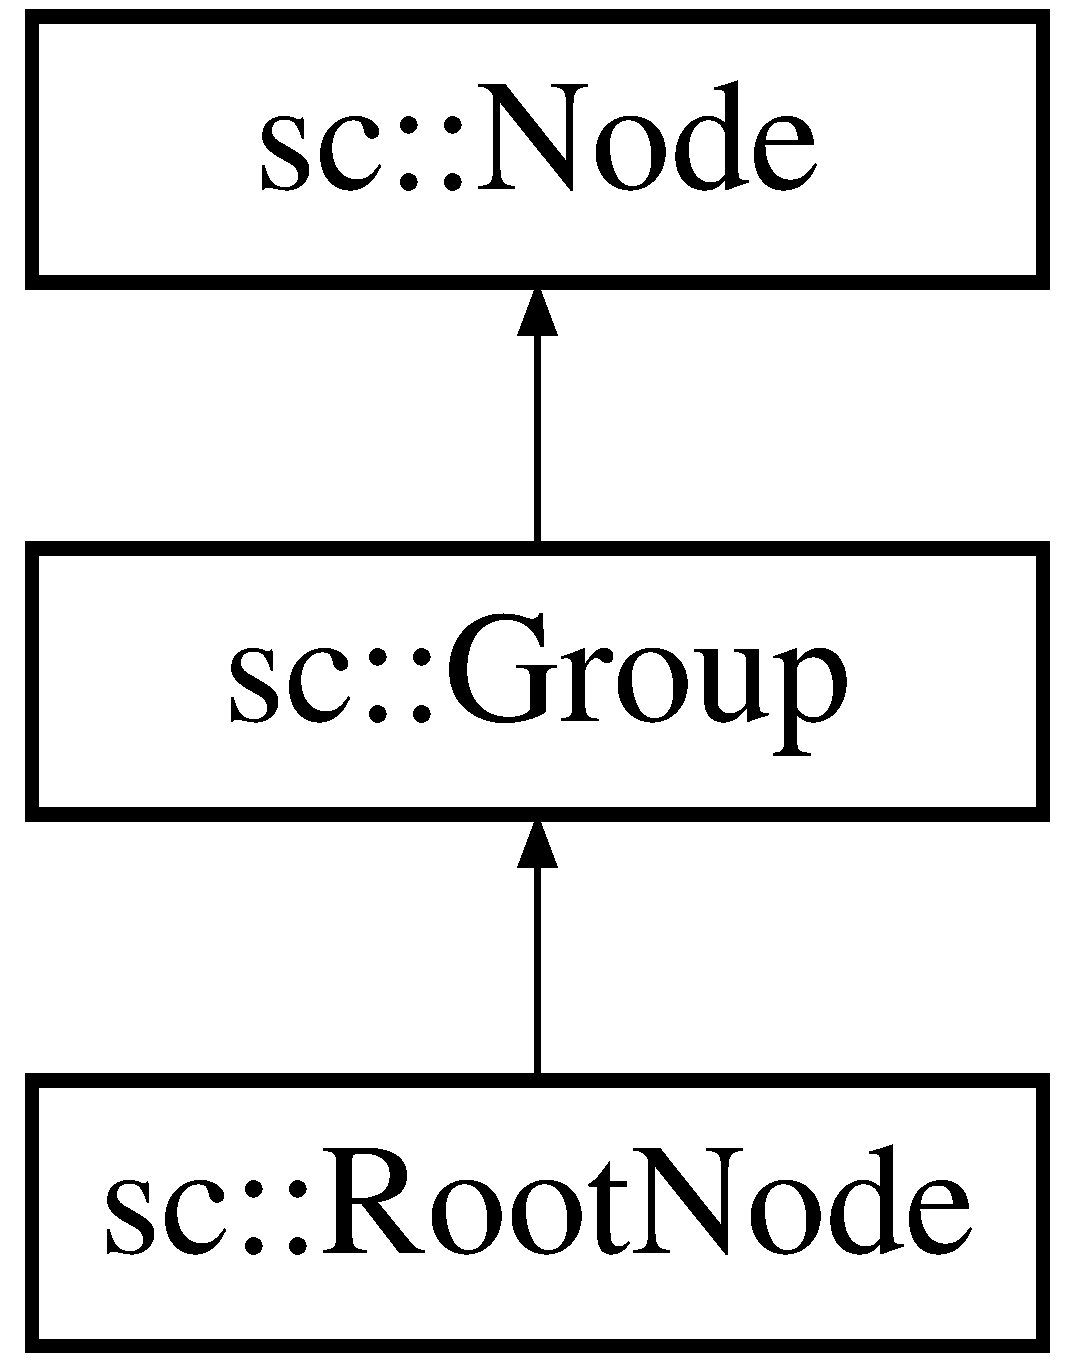
\includegraphics[height=3.000000cm]{classsc_1_1Group}
\end{center}
\end{figure}
\subsection*{Public Member Functions}
\begin{DoxyCompactItemize}
\item 
\hyperlink{classsc_1_1Group_a091ad4312c030cd0cde27ef2aac7cbbd}{Group} (\hyperlink{classsc_1_1SCServer}{S\-C\-Server} $\ast$other, const std\-::string \&name, int id\-\_\-, int add\-Action=T\-O\-\_\-\-H\-E\-A\-D, int target=D\-E\-F\-A\-U\-L\-T\-\_\-\-G\-R\-O\-U\-P)
\item 
\hypertarget{classsc_1_1Group_a10466798a0549aa877931be7ad226d63}{\hyperlink{classsc_1_1Group_a10466798a0549aa877931be7ad226d63}{$\sim$\-Group} ()}\label{classsc_1_1Group_a10466798a0549aa877931be7ad226d63}

\begin{DoxyCompactList}\small\item\em Destructor. \end{DoxyCompactList}\item 
void \hyperlink{classsc_1_1Group_a779027324b685e67cabdc751fdc58ff2}{free\-All\-Synths} ()
\item 
void \hyperlink{classsc_1_1Group_af1a8e311e5009f5d1c72f189fa146fbf}{deep\-Free\-All\-Synths} ()
\end{DoxyCompactItemize}


\subsection{Detailed Description}
This class represents a client-\/side version of a server group. 

\subsection{Constructor \& Destructor Documentation}
\hypertarget{classsc_1_1Group_a091ad4312c030cd0cde27ef2aac7cbbd}{\index{sc\-::\-Group@{sc\-::\-Group}!Group@{Group}}
\index{Group@{Group}!sc::Group@{sc\-::\-Group}}
\subsubsection[{Group}]{\setlength{\rightskip}{0pt plus 5cm}sc\-::\-Group\-::\-Group (
\begin{DoxyParamCaption}
\item[{{\bf S\-C\-Server} $\ast$}]{other, }
\item[{const std\-::string \&}]{name, }
\item[{int}]{id\-\_\-, }
\item[{int}]{add\-Action = {\ttfamily TO\-\_\-HEAD}, }
\item[{int}]{target = {\ttfamily DEFAULT\-\_\-GROUP}}
\end{DoxyParamCaption}
)}}\label{classsc_1_1Group_a091ad4312c030cd0cde27ef2aac7cbbd}
Create a \hyperlink{classsc_1_1Group}{Group} with a user defined name, id, add\-Action, and target If no add\-Action is specified, this \hyperlink{classsc_1_1Group}{Group} is added to the head of target group If no target group is specified, this \hyperlink{classsc_1_1Synth}{Synth} is added to the Default \hyperlink{classsc_1_1Group}{Group} 
\begin{DoxyParams}[1]{Parameters}
\mbox{\tt in}  & {\em S\-C\-Server\&} & \hyperlink{classsc_1_1SCServer}{S\-C\-Server} instance \\
\hline
\mbox{\tt in}  & {\em const} & std\-::string\& Name \\
\hline
\mbox{\tt in}  & {\em int} & Id \\
\hline
\mbox{\tt in}  & {\em int} & Add Action \\
\hline
\mbox{\tt in}  & {\em int} & Target \hyperlink{classsc_1_1Group}{Group} \\
\hline
\end{DoxyParams}


\subsection{Member Function Documentation}
\hypertarget{classsc_1_1Group_af1a8e311e5009f5d1c72f189fa146fbf}{\index{sc\-::\-Group@{sc\-::\-Group}!deep\-Free\-All\-Synths@{deep\-Free\-All\-Synths}}
\index{deep\-Free\-All\-Synths@{deep\-Free\-All\-Synths}!sc::Group@{sc\-::\-Group}}
\subsubsection[{deep\-Free\-All\-Synths}]{\setlength{\rightskip}{0pt plus 5cm}void sc\-::\-Group\-::deep\-Free\-All\-Synths (
\begin{DoxyParamCaption}
{}
\end{DoxyParamCaption}
)}}\label{classsc_1_1Group_af1a8e311e5009f5d1c72f189fa146fbf}
Free all Nodes in this \hyperlink{classsc_1_1Group}{Group} and in all Sub-\/\-Groups 
\begin{DoxyParams}[1]{Parameters}
\mbox{\tt in}  & {\em S\-C\-Server\&} & \hyperlink{classsc_1_1SCServer}{S\-C\-Server} instance \\
\hline
\end{DoxyParams}
\hypertarget{classsc_1_1Group_a779027324b685e67cabdc751fdc58ff2}{\index{sc\-::\-Group@{sc\-::\-Group}!free\-All\-Synths@{free\-All\-Synths}}
\index{free\-All\-Synths@{free\-All\-Synths}!sc::Group@{sc\-::\-Group}}
\subsubsection[{free\-All\-Synths}]{\setlength{\rightskip}{0pt plus 5cm}void sc\-::\-Group\-::free\-All\-Synths (
\begin{DoxyParamCaption}
{}
\end{DoxyParamCaption}
)}}\label{classsc_1_1Group_a779027324b685e67cabdc751fdc58ff2}
Free all Nodes in this \hyperlink{classsc_1_1Group}{Group} 
\begin{DoxyParams}[1]{Parameters}
\mbox{\tt in}  & {\em S\-C\-Server\&} & \hyperlink{classsc_1_1SCServer}{S\-C\-Server} instance \\
\hline
\end{DoxyParams}


The documentation for this class was generated from the following file\-:\begin{DoxyCompactItemize}
\item 
include/\hyperlink{Node_8hpp}{Node.\-hpp}\end{DoxyCompactItemize}

\hypertarget{classsc_1_1Node}{\section{sc\-:\-:Node Class Reference}
\label{classsc_1_1Node}\index{sc\-::\-Node@{sc\-::\-Node}}
}


This class represents a client-\/side version of a server node (\hyperlink{classsc_1_1Synth}{Synth} or \hyperlink{classsc_1_1Group}{Group})  




{\ttfamily \#include $<$Node.\-hpp$>$}

Inheritance diagram for sc\-:\-:Node\-:\begin{figure}[H]
\begin{center}
\leavevmode
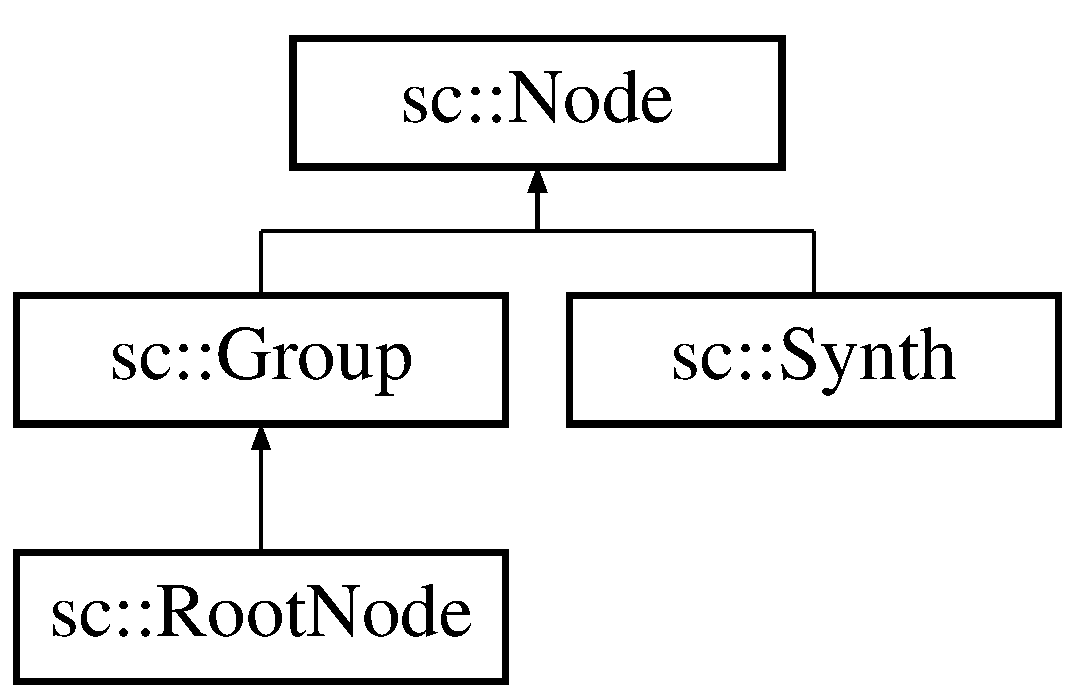
\includegraphics[height=3.000000cm]{classsc_1_1Node}
\end{center}
\end{figure}
\subsection*{Public Member Functions}
\begin{DoxyCompactItemize}
\item 
\hyperlink{classsc_1_1Node_aebe6b60f2f6312495480d0a2e01c7efa}{Node} (\hyperlink{classsc_1_1SCServer}{S\-C\-Server} $\ast$other, const std\-::string \&def\-Name, int id\-\_\-)
\item 
\hypertarget{classsc_1_1Node_a12fa05f533aa00bf553b9a46db1fcd45}{\hyperlink{classsc_1_1Node_a12fa05f533aa00bf553b9a46db1fcd45}{$\sim$\-Node} ()}\label{classsc_1_1Node_a12fa05f533aa00bf553b9a46db1fcd45}

\begin{DoxyCompactList}\small\item\em Destructor. \end{DoxyCompactList}\item 
int \hyperlink{classsc_1_1Node_ae9fd8f68186f13b1402c542192b98e63}{get\-Id} () const 
\item 
\hypertarget{classsc_1_1Node_a21719bc1c64204fe09351e42f2dc4894}{void \hyperlink{classsc_1_1Node_a21719bc1c64204fe09351e42f2dc4894}{run} ()}\label{classsc_1_1Node_a21719bc1c64204fe09351e42f2dc4894}

\begin{DoxyCompactList}\small\item\em Command the server to run this \hyperlink{classsc_1_1Node}{Node}. \end{DoxyCompactList}\item 
\hypertarget{classsc_1_1Node_a4e39d4f8bfd05a8f710184ac7153b269}{void \hyperlink{classsc_1_1Node_a4e39d4f8bfd05a8f710184ac7153b269}{pause} ()}\label{classsc_1_1Node_a4e39d4f8bfd05a8f710184ac7153b269}

\begin{DoxyCompactList}\small\item\em Command the server to stop this \hyperlink{classsc_1_1Node}{Node}. \end{DoxyCompactList}\item 
\hypertarget{classsc_1_1Node_a5e78540a85cd945dabb0f5cf9571fd03}{void \hyperlink{classsc_1_1Node_a5e78540a85cd945dabb0f5cf9571fd03}{free} ()}\label{classsc_1_1Node_a5e78540a85cd945dabb0f5cf9571fd03}

\begin{DoxyCompactList}\small\item\em Command the server to free this \hyperlink{classsc_1_1Node}{Node}. \end{DoxyCompactList}\item 
bool \hyperlink{classsc_1_1Node_a551ece6304c94df930d59bc6fe13b6ba}{is\-Playing} () const 
\item 
bool \hyperlink{classsc_1_1Node_a3aa0c120ba5a7983e7b0e2f8ba6ace73}{is\-Running} () const 
\item 
bool \hyperlink{classsc_1_1Node_afc9868d6f3186648f4ab178929531003}{get\-Manually\-Freed} () const 
\item 
std\-::string \hyperlink{classsc_1_1Node_a7b6432f40057dc5f8f4d860defe3889a}{get\-Def\-Name} () const 
\item 
\hyperlink{classsc_1_1SCServer}{S\-C\-Server} $\ast$ \hyperlink{classsc_1_1Node_ae62cc58163364d644cfa9df669594d4f}{get\-Client\-Server} () const 
\item 
\hypertarget{classsc_1_1Node_a545de1cb729a6c7458396984f743b53f}{void \hyperlink{classsc_1_1Node_a545de1cb729a6c7458396984f743b53f}{sync} ()}\label{classsc_1_1Node_a545de1cb729a6c7458396984f743b53f}

\begin{DoxyCompactList}\small\item\em Query the server for this \hyperlink{classsc_1_1Node}{Node}. \end{DoxyCompactList}\end{DoxyCompactItemize}
\begin{Indent}{\bf Control and Bus Mapping Functions}\par
\begin{DoxyCompactItemize}
\item 
void \hyperlink{classsc_1_1Node_af29f544918afd0a212450c189e525224}{set} (std\-::map$<$ std\-::string, float $>$ \&control\-Vals)
\item 
void \hyperlink{classsc_1_1Node_a66e25d5cdfe57e7b9930a121fcc1d3ce}{setn} (std\-::map$<$ std\-::string, float\mbox{[}$\,$\mbox{]}$>$ \&control\-Ranges)
\item 
void \hyperlink{classsc_1_1Node_ac1c3c7c888c46c4f731862871d2dea7b}{bus\-Map} (std\-::map$<$ std\-::string, \hyperlink{classsc_1_1Bus}{Bus} $>$ \&map)
\end{DoxyCompactItemize}
\end{Indent}


\subsection{Detailed Description}
This class represents a client-\/side version of a server node (\hyperlink{classsc_1_1Synth}{Synth} or \hyperlink{classsc_1_1Group}{Group}) 

\subsection{Constructor \& Destructor Documentation}
\hypertarget{classsc_1_1Node_aebe6b60f2f6312495480d0a2e01c7efa}{\index{sc\-::\-Node@{sc\-::\-Node}!Node@{Node}}
\index{Node@{Node}!sc::Node@{sc\-::\-Node}}
\subsubsection[{Node}]{\setlength{\rightskip}{0pt plus 5cm}sc\-::\-Node\-::\-Node (
\begin{DoxyParamCaption}
\item[{{\bf S\-C\-Server} $\ast$}]{other, }
\item[{const std\-::string \&}]{def\-Name, }
\item[{int}]{id\-\_\-}
\end{DoxyParamCaption}
)}}\label{classsc_1_1Node_aebe6b60f2f6312495480d0a2e01c7efa}
Create a \hyperlink{classsc_1_1Node}{Node} with a user defined name and Id 
\begin{DoxyParams}[1]{Parameters}
\mbox{\tt in}  & {\em const} & std\-::string\& Name \\
\hline
\mbox{\tt in}  & {\em int} & Id \\
\hline
\end{DoxyParams}


\subsection{Member Function Documentation}
\hypertarget{classsc_1_1Node_ac1c3c7c888c46c4f731862871d2dea7b}{\index{sc\-::\-Node@{sc\-::\-Node}!bus\-Map@{bus\-Map}}
\index{bus\-Map@{bus\-Map}!sc::Node@{sc\-::\-Node}}
\subsubsection[{bus\-Map}]{\setlength{\rightskip}{0pt plus 5cm}void sc\-::\-Node\-::bus\-Map (
\begin{DoxyParamCaption}
\item[{std\-::map$<$ std\-::string, {\bf Bus} $>$ \&}]{map}
\end{DoxyParamCaption}
)}}\label{classsc_1_1Node_ac1c3c7c888c46c4f731862871d2dea7b}
Set this \hyperlink{classsc_1_1Node}{Node} with specified bus mappings 
\begin{DoxyParams}[1]{Parameters}
\mbox{\tt in}  & {\em S\-C\-Server\&} & \hyperlink{classsc_1_1SCServer}{S\-C\-Server} instance \\
\hline
\mbox{\tt in}  & {\em std\-::map$<$std\-::string,Bus$>$\&} & map \\
\hline
\end{DoxyParams}
\hypertarget{classsc_1_1Node_ae62cc58163364d644cfa9df669594d4f}{\index{sc\-::\-Node@{sc\-::\-Node}!get\-Client\-Server@{get\-Client\-Server}}
\index{get\-Client\-Server@{get\-Client\-Server}!sc::Node@{sc\-::\-Node}}
\subsubsection[{get\-Client\-Server}]{\setlength{\rightskip}{0pt plus 5cm}{\bf S\-C\-Server}$\ast$ sc\-::\-Node\-::get\-Client\-Server (
\begin{DoxyParamCaption}
{}
\end{DoxyParamCaption}
) const\hspace{0.3cm}{\ttfamily [inline]}}}\label{classsc_1_1Node_ae62cc58163364d644cfa9df669594d4f}
Return this \hyperlink{classsc_1_1Node}{Node}'s \hyperlink{classsc_1_1SCServer}{S\-C\-Server} pointer \begin{DoxyReturn}{Returns}
cs 
\end{DoxyReturn}
\hypertarget{classsc_1_1Node_a7b6432f40057dc5f8f4d860defe3889a}{\index{sc\-::\-Node@{sc\-::\-Node}!get\-Def\-Name@{get\-Def\-Name}}
\index{get\-Def\-Name@{get\-Def\-Name}!sc::Node@{sc\-::\-Node}}
\subsubsection[{get\-Def\-Name}]{\setlength{\rightskip}{0pt plus 5cm}std\-::string sc\-::\-Node\-::get\-Def\-Name (
\begin{DoxyParamCaption}
{}
\end{DoxyParamCaption}
) const\hspace{0.3cm}{\ttfamily [inline]}}}\label{classsc_1_1Node_a7b6432f40057dc5f8f4d860defe3889a}
Returns the name of this \hyperlink{classsc_1_1Node}{Node} \begin{DoxyReturn}{Returns}
def\-Name 
\end{DoxyReturn}
\hypertarget{classsc_1_1Node_ae9fd8f68186f13b1402c542192b98e63}{\index{sc\-::\-Node@{sc\-::\-Node}!get\-Id@{get\-Id}}
\index{get\-Id@{get\-Id}!sc::Node@{sc\-::\-Node}}
\subsubsection[{get\-Id}]{\setlength{\rightskip}{0pt plus 5cm}int sc\-::\-Node\-::get\-Id (
\begin{DoxyParamCaption}
{}
\end{DoxyParamCaption}
) const\hspace{0.3cm}{\ttfamily [inline]}}}\label{classsc_1_1Node_ae9fd8f68186f13b1402c542192b98e63}
Returns the Id of this \hyperlink{classsc_1_1Node}{Node} \begin{DoxyReturn}{Returns}
id 
\end{DoxyReturn}
\hypertarget{classsc_1_1Node_afc9868d6f3186648f4ab178929531003}{\index{sc\-::\-Node@{sc\-::\-Node}!get\-Manually\-Freed@{get\-Manually\-Freed}}
\index{get\-Manually\-Freed@{get\-Manually\-Freed}!sc::Node@{sc\-::\-Node}}
\subsubsection[{get\-Manually\-Freed}]{\setlength{\rightskip}{0pt plus 5cm}bool sc\-::\-Node\-::get\-Manually\-Freed (
\begin{DoxyParamCaption}
{}
\end{DoxyParamCaption}
) const\hspace{0.3cm}{\ttfamily [inline]}}}\label{classsc_1_1Node_afc9868d6f3186648f4ab178929531003}
Returns true if the \hyperlink{classsc_1_1Node}{Node} was freed from the server by calling \hyperlink{classsc_1_1Node_a5e78540a85cd945dabb0f5cf9571fd03}{free()} B\-E\-F\-O\-R\-E the destructor of this \hyperlink{classsc_1_1Node}{Node} is called \begin{DoxyReturn}{Returns}
true if freed from server with \hyperlink{classsc_1_1Node_a5e78540a85cd945dabb0f5cf9571fd03}{free()} prior to destruction 
\end{DoxyReturn}
\hypertarget{classsc_1_1Node_a551ece6304c94df930d59bc6fe13b6ba}{\index{sc\-::\-Node@{sc\-::\-Node}!is\-Playing@{is\-Playing}}
\index{is\-Playing@{is\-Playing}!sc::Node@{sc\-::\-Node}}
\subsubsection[{is\-Playing}]{\setlength{\rightskip}{0pt plus 5cm}bool sc\-::\-Node\-::is\-Playing (
\begin{DoxyParamCaption}
{}
\end{DoxyParamCaption}
) const\hspace{0.3cm}{\ttfamily [inline]}}}\label{classsc_1_1Node_a551ece6304c94df930d59bc6fe13b6ba}
Returns true if this \hyperlink{classsc_1_1Node}{Node} is currently playing, else false \begin{DoxyReturn}{Returns}
true if currently playing, else false 
\end{DoxyReturn}
\hypertarget{classsc_1_1Node_a3aa0c120ba5a7983e7b0e2f8ba6ace73}{\index{sc\-::\-Node@{sc\-::\-Node}!is\-Running@{is\-Running}}
\index{is\-Running@{is\-Running}!sc::Node@{sc\-::\-Node}}
\subsubsection[{is\-Running}]{\setlength{\rightskip}{0pt plus 5cm}bool sc\-::\-Node\-::is\-Running (
\begin{DoxyParamCaption}
{}
\end{DoxyParamCaption}
) const\hspace{0.3cm}{\ttfamily [inline]}}}\label{classsc_1_1Node_a3aa0c120ba5a7983e7b0e2f8ba6ace73}
Returns true if this \hyperlink{classsc_1_1Node}{Node} is currently running, else false \begin{DoxyReturn}{Returns}
true if currently running, else false 
\end{DoxyReturn}
\hypertarget{classsc_1_1Node_af29f544918afd0a212450c189e525224}{\index{sc\-::\-Node@{sc\-::\-Node}!set@{set}}
\index{set@{set}!sc::Node@{sc\-::\-Node}}
\subsubsection[{set}]{\setlength{\rightskip}{0pt plus 5cm}void sc\-::\-Node\-::set (
\begin{DoxyParamCaption}
\item[{std\-::map$<$ std\-::string, float $>$ \&}]{control\-Vals}
\end{DoxyParamCaption}
)}}\label{classsc_1_1Node_af29f544918afd0a212450c189e525224}
Set this \hyperlink{classsc_1_1Node}{Node} with specified control values 
\begin{DoxyParams}[1]{Parameters}
\mbox{\tt in}  & {\em S\-C\-Server\&} & \hyperlink{classsc_1_1SCServer}{S\-C\-Server} instance \\
\hline
\mbox{\tt in}  & {\em std\-::map$<$std\-::string,float$>$\&} & Control Values \\
\hline
\end{DoxyParams}
\hypertarget{classsc_1_1Node_a66e25d5cdfe57e7b9930a121fcc1d3ce}{\index{sc\-::\-Node@{sc\-::\-Node}!setn@{setn}}
\index{setn@{setn}!sc::Node@{sc\-::\-Node}}
\subsubsection[{setn}]{\setlength{\rightskip}{0pt plus 5cm}void sc\-::\-Node\-::setn (
\begin{DoxyParamCaption}
\item[{std\-::map$<$ std\-::string, float\mbox{[}$\,$\mbox{]}$>$ \&}]{control\-Ranges}
\end{DoxyParamCaption}
)}}\label{classsc_1_1Node_a66e25d5cdfe57e7b9930a121fcc1d3ce}
Set this \hyperlink{classsc_1_1Node}{Node} with specified control range values 
\begin{DoxyParams}[1]{Parameters}
\mbox{\tt in}  & {\em S\-C\-Server\&} & \hyperlink{classsc_1_1SCServer}{S\-C\-Server} instance \\
\hline
\mbox{\tt in}  & {\em std\-::map$<$std\-::string,float\mbox{[}$\,$\mbox{]}$>$\&} & Control Ranges \\
\hline
\end{DoxyParams}


The documentation for this class was generated from the following file\-:\begin{DoxyCompactItemize}
\item 
include/\hyperlink{Node_8hpp}{Node.\-hpp}\end{DoxyCompactItemize}

\hypertarget{classsc_1_1RootNode}{\section{sc\-:\-:Root\-Node Class Reference}
\label{classsc_1_1RootNode}\index{sc\-::\-Root\-Node@{sc\-::\-Root\-Node}}
}


This class represents a client-\/side version of a server root node.  




{\ttfamily \#include $<$Node.\-hpp$>$}

Inheritance diagram for sc\-:\-:Root\-Node\-:\begin{figure}[H]
\begin{center}
\leavevmode
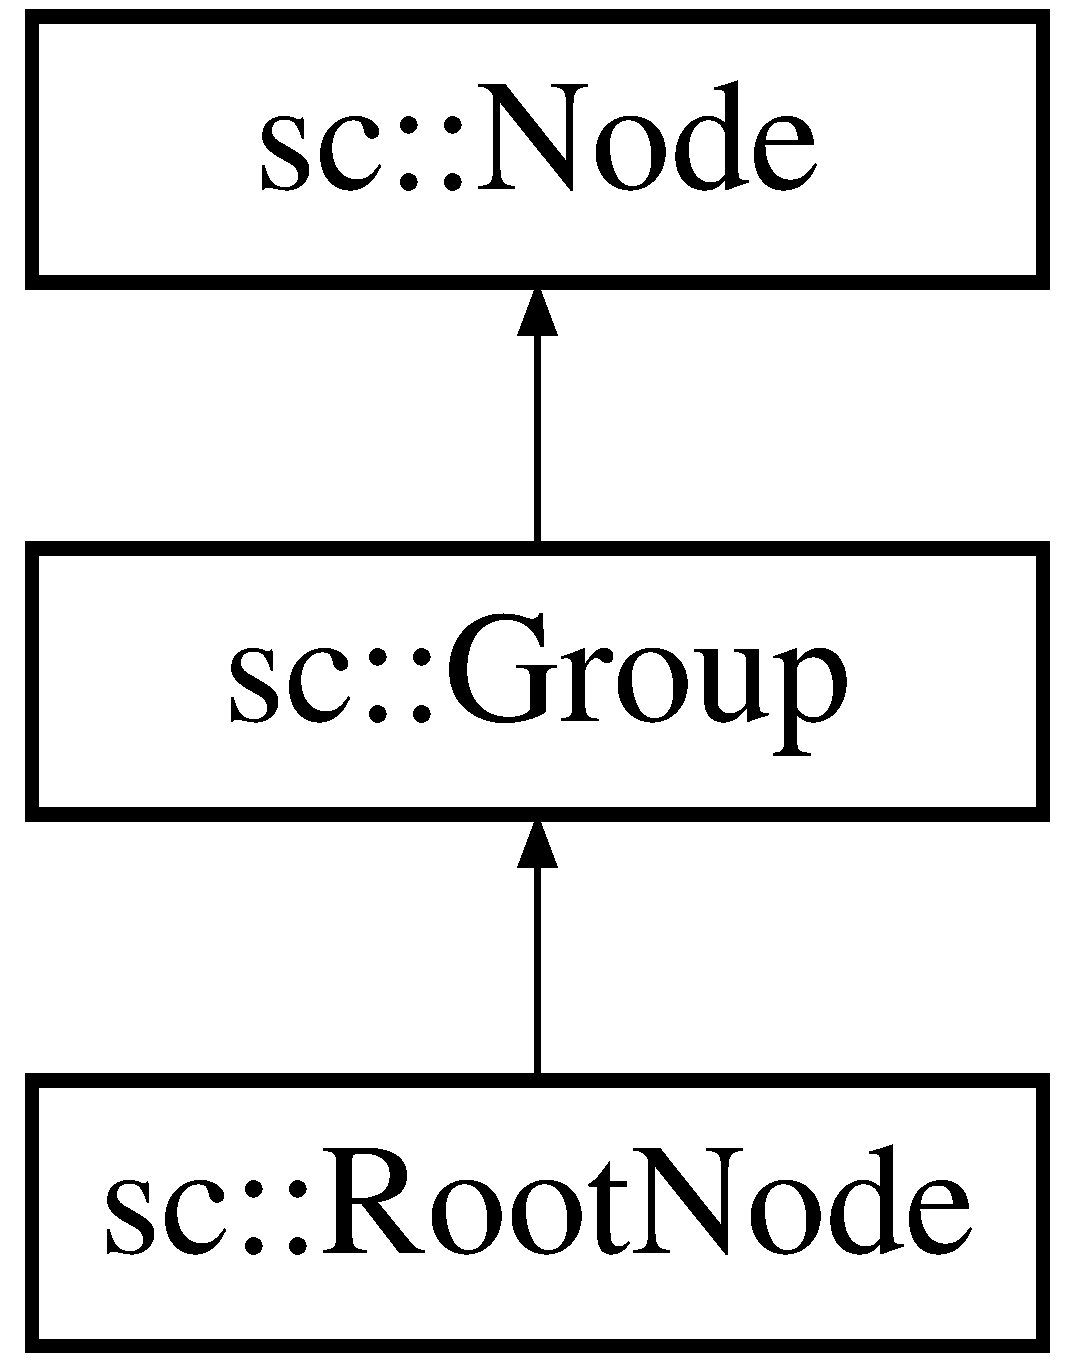
\includegraphics[height=3.000000cm]{classsc_1_1RootNode}
\end{center}
\end{figure}
\subsection*{Public Member Functions}
\begin{DoxyCompactItemize}
\item 
\hyperlink{classsc_1_1RootNode_a6ce777b07fdd3ea007dee967d9aadb3d}{Root\-Node} (\hyperlink{classsc_1_1SCServer}{S\-C\-Server} $\ast$other)
\item 
\hypertarget{classsc_1_1RootNode_a6dc8c84f94d46d7586cbcbd059b64a41}{\hyperlink{classsc_1_1RootNode_a6dc8c84f94d46d7586cbcbd059b64a41}{$\sim$\-Root\-Node} ()}\label{classsc_1_1RootNode_a6dc8c84f94d46d7586cbcbd059b64a41}

\begin{DoxyCompactList}\small\item\em Destructor. \end{DoxyCompactList}\end{DoxyCompactItemize}


\subsection{Detailed Description}
This class represents a client-\/side version of a server root node. 

\subsection{Constructor \& Destructor Documentation}
\hypertarget{classsc_1_1RootNode_a6ce777b07fdd3ea007dee967d9aadb3d}{\index{sc\-::\-Root\-Node@{sc\-::\-Root\-Node}!Root\-Node@{Root\-Node}}
\index{Root\-Node@{Root\-Node}!sc::RootNode@{sc\-::\-Root\-Node}}
\subsubsection[{Root\-Node}]{\setlength{\rightskip}{0pt plus 5cm}sc\-::\-Root\-Node\-::\-Root\-Node (
\begin{DoxyParamCaption}
\item[{{\bf S\-C\-Server} $\ast$}]{other}
\end{DoxyParamCaption}
)}}\label{classsc_1_1RootNode_a6ce777b07fdd3ea007dee967d9aadb3d}
Create a Root \hyperlink{classsc_1_1Node}{Node} 
\begin{DoxyParams}[1]{Parameters}
\mbox{\tt in}  & {\em S\-C\-Server\&} & \hyperlink{classsc_1_1SCServer}{S\-C\-Server} instance \\
\hline
\end{DoxyParams}


The documentation for this class was generated from the following file\-:\begin{DoxyCompactItemize}
\item 
include/\hyperlink{Node_8hpp}{Node.\-hpp}\end{DoxyCompactItemize}

\hypertarget{classsc_1_1SCServer}{\section{sc\-:\-:S\-C\-Server Class Reference}
\label{classsc_1_1SCServer}\index{sc\-::\-S\-C\-Server@{sc\-::\-S\-C\-Server}}
}


This class represents a client-\/side version of scsynth, the Super\-Collider audio server.  




{\ttfamily \#include $<$S\-C\-Server.\-hpp$>$}

\subsection*{Public Member Functions}
\begin{DoxyCompactItemize}
\item 
\hypertarget{classsc_1_1SCServer_aaec728927e957f6190682760bb191661}{\hyperlink{classsc_1_1SCServer_aaec728927e957f6190682760bb191661}{S\-C\-Server} ()}\label{classsc_1_1SCServer_aaec728927e957f6190682760bb191661}

\begin{DoxyCompactList}\small\item\em Create a default \hyperlink{classsc_1_1SCServer}{S\-C\-Server}. \end{DoxyCompactList}\item 
\hyperlink{classsc_1_1SCServer_a5be05ff132abc5927e5ce3423978238d}{S\-C\-Server} (const std\-::string \&name, const char $\ast$host, const char $\ast$port, const std\-::string \&synth\-Def\-Dir)
\item 
\hypertarget{classsc_1_1SCServer_a673ad092d5d67da3be3aa04f2ac19ec6}{\hyperlink{classsc_1_1SCServer_a673ad092d5d67da3be3aa04f2ac19ec6}{$\sim$\-S\-C\-Server} ()}\label{classsc_1_1SCServer_a673ad092d5d67da3be3aa04f2ac19ec6}

\begin{DoxyCompactList}\small\item\em Destructor. \end{DoxyCompactList}\item 
void \hyperlink{classsc_1_1SCServer_af37066ecf33f14b2d26be8b455026f73}{remove\-Buffer} (void $\ast$buffer)
\item 
void \hyperlink{classsc_1_1SCServer_a0b1f014764c249411c7b033b5cd2aca3}{add\-Node} (void $\ast$node)
\item 
void \hyperlink{classsc_1_1SCServer_ac024296f9c382e9f2bb00bc765695565}{remove\-Node} (void $\ast$node)
\end{DoxyCompactItemize}
\begin{Indent}{\bf General System Functions}\par
\begin{DoxyCompactItemize}
\item 
std\-::string \hyperlink{classsc_1_1SCServer_a663f38241749842d676f29463edb9c22}{get\-Name} () const 
\item 
int \hyperlink{classsc_1_1SCServer_ad1194f90f47d7ce50390953bd785b75b}{next\-Node\-Id} ()
\item 
int \hyperlink{classsc_1_1SCServer_aec43a53cc18c49dae4066b4bf85e2067}{next\-Buffer\-Num} ()
\item 
void \hyperlink{classsc_1_1SCServer_ada96ef4c5ea8747899a6db947ec33363}{dump\-O\-S\-C} (int toggle)
\item 
\hypertarget{classsc_1_1SCServer_ac884ae7c3f2791f6b959818c8c2fbe10}{void \hyperlink{classsc_1_1SCServer_ac884ae7c3f2791f6b959818c8c2fbe10}{print\-Current\-Node\-Ids} ()}\label{classsc_1_1SCServer_ac884ae7c3f2791f6b959818c8c2fbe10}

\begin{DoxyCompactList}\small\item\em Print current \hyperlink{classsc_1_1Node}{Node} ids associated with this instance. \end{DoxyCompactList}\item 
\hypertarget{classsc_1_1SCServer_ad057f9ca7dab818c259f95f41e3a575e}{void \hyperlink{classsc_1_1SCServer_ad057f9ca7dab818c259f95f41e3a575e}{query\-Node\-Tree} ()}\label{classsc_1_1SCServer_ad057f9ca7dab818c259f95f41e3a575e}

\begin{DoxyCompactList}\small\item\em Command server to print current \hyperlink{classsc_1_1Node}{Node} tree. \end{DoxyCompactList}\item 
\hypertarget{classsc_1_1SCServer_a775f079ad6a09282356ae161b186e345}{void \hyperlink{classsc_1_1SCServer_a775f079ad6a09282356ae161b186e345}{query\-Node} (int node\-Id)}\label{classsc_1_1SCServer_a775f079ad6a09282356ae161b186e345}

\begin{DoxyCompactList}\small\item\em Query a specific node for its info on the server. \end{DoxyCompactList}\item 
\hypertarget{classsc_1_1SCServer_a9418167a772b6f0f4495c262938277b9}{void \hyperlink{classsc_1_1SCServer_a9418167a772b6f0f4495c262938277b9}{status} ()}\label{classsc_1_1SCServer_a9418167a772b6f0f4495c262938277b9}

\begin{DoxyCompactList}\small\item\em Send /status command to server, replies with /status\-\_\-info. \end{DoxyCompactList}\item 
bool \hyperlink{classsc_1_1SCServer_ac8d0c043f3e055778304fd1d34cf75dc}{notify} (int toggle)
\item 
bool \hyperlink{classsc_1_1SCServer_a6ae0d1f3acafa5c3421725426d0beb96}{quit} ()
\end{DoxyCompactItemize}
\end{Indent}
\begin{Indent}{\bf Node Functions}\par
\begin{DoxyCompactItemize}
\item 
bool \hyperlink{classsc_1_1SCServer_abb82887e9757e1fa0df687344db73ba5}{load\-Synth\-Def} (const std\-::string \&synth\-Def\-Name)
\item 
bool \hyperlink{classsc_1_1SCServer_adc5a4cc11762007cfcad404f5eaf2699}{load\-Synth\-Def\-Directory} (const std\-::string \&synth\-Def\-Dir)
\item 
void \hyperlink{classsc_1_1SCServer_aee46c819d9e4e146e0a53d06eccd7a95}{create\-Node} (int node\-Id, int add\-Action=T\-O\-\_\-\-H\-E\-A\-D, int target=D\-E\-F\-A\-U\-L\-T\-\_\-\-G\-R\-O\-U\-P, int type=S\-Y\-N\-T\-H)
\item 
void \hyperlink{classsc_1_1SCServer_a2ac7cabe7d491c6ecd9193635f25aa77}{create\-Node} (const std\-::string \&name, int node\-Id, int add\-Action=T\-O\-\_\-\-H\-E\-A\-D, int target=D\-E\-F\-A\-U\-L\-T\-\_\-\-G\-R\-O\-U\-P, int type=S\-Y\-N\-T\-H)
\item 
void \hyperlink{classsc_1_1SCServer_ac94bcf8ddce587e836631a23f1059088}{create\-Synth} (const std\-::string \&name, int node\-Id, int add\-Action=T\-O\-\_\-\-H\-E\-A\-D, int target=D\-E\-F\-A\-U\-L\-T\-\_\-\-G\-R\-O\-U\-P)
\item 
void \hyperlink{classsc_1_1SCServer_ab8b14584833941f06693f097d381e551}{create\-Paused\-Synth} (const std\-::string \&name, int node\-Id, int add\-Action=T\-O\-\_\-\-H\-E\-A\-D, int target=D\-E\-F\-A\-U\-L\-T\-\_\-\-G\-R\-O\-U\-P)
\item 
void \hyperlink{classsc_1_1SCServer_a7baac4a701937c38d421aa4ed265350b}{create\-Synth} (const std\-::string \&name, int node\-Id, std\-::map$<$ std\-::string, float $>$ \&args, int add\-Action=T\-O\-\_\-\-H\-E\-A\-D, int target=D\-E\-F\-A\-U\-L\-T\-\_\-\-G\-R\-O\-U\-P)
\item 
void \hyperlink{classsc_1_1SCServer_a0cc7ed517234f06d42d24f4576201155}{create\-Paused\-Synth} (const std\-::string \&name, int node\-Id, std\-::map$<$ std\-::string, float $>$ \&args, int add\-Action=T\-O\-\_\-\-H\-E\-A\-D, int target=D\-E\-F\-A\-U\-L\-T\-\_\-\-G\-R\-O\-U\-P)
\item 
void \hyperlink{classsc_1_1SCServer_a9aab99e02f70516217b320fc6c453951}{create\-Group} (int node\-Id, int add\-Action=T\-O\-\_\-\-H\-E\-A\-D, int target=D\-E\-F\-A\-U\-L\-T\-\_\-\-G\-R\-O\-U\-P)
\item 
void \hyperlink{classsc_1_1SCServer_a22b904f4d18160178d8dff424579b821}{run\-Node} (int node\-Id, int flag)
\item 
void \hyperlink{classsc_1_1SCServer_ac2c5c3092d2ba8781f2bb0f91ccaf7cd}{free\-Node} (int node\-I\-D)
\item 
void \hyperlink{classsc_1_1SCServer_a41296f0d6d948ada6a7509e767cabeb0}{set\-Node\-Controls} (int node\-Id, std\-::map$<$ std\-::string, float $>$ \&control\-Vals)
\item 
void \hyperlink{classsc_1_1SCServer_a8e5460d2e8b184f35c648c688e1b31f3}{free\-All\-Synths} (int group\-Id)
\item 
void \hyperlink{classsc_1_1SCServer_a8739643e0aa244661e41f229aca329ba}{deep\-Free\-All\-Synths} (int group\-Id)
\end{DoxyCompactItemize}
\end{Indent}
\begin{Indent}{\bf Buffer Functions}\par
\begin{DoxyCompactItemize}
\item 
bool \hyperlink{classsc_1_1SCServer_a4a93b0de3cabaed3a4c32327f08b1d58}{alloc\-Buffer} (int buf\-Num, int num\-Frames, int num\-Chans)
\item 
bool \hyperlink{classsc_1_1SCServer_a5e89d3374fd704cea3110894c9c62b07}{free\-Buffer} (int buf\-Num)
\item 
\hypertarget{classsc_1_1SCServer_a00ce072fc88c75aa6885da7a652701a9}{void {\bfseries free\-Buffer\-\_\-no\-\_\-reply} (int buf\-Num)}\label{classsc_1_1SCServer_a00ce072fc88c75aa6885da7a652701a9}

\item 
bool \hyperlink{classsc_1_1SCServer_a3d03cd0dd763f2f575d6a84da55609bf}{alloc\-Read\-Buffer} (int buf\-Num, const std\-::string \&file\-Path, int start\-File\-Frame=0, int num\-Frames=-\/1)
\item 
void \hyperlink{classsc_1_1SCServer_acbd0a404dbd4e2cc98e46d088643908b}{query\-Buffer} (int buf\-Num)
\item 
void \hyperlink{classsc_1_1SCServer_ade0d2a48713efbce6494ad0bae42a839}{add\-Buffer} (void $\ast$buffer)
\end{DoxyCompactItemize}
\end{Indent}


\subsection{Detailed Description}
This class represents a client-\/side version of scsynth, the Super\-Collider audio server. 

\subsection{Constructor \& Destructor Documentation}
\hypertarget{classsc_1_1SCServer_a5be05ff132abc5927e5ce3423978238d}{\index{sc\-::\-S\-C\-Server@{sc\-::\-S\-C\-Server}!S\-C\-Server@{S\-C\-Server}}
\index{S\-C\-Server@{S\-C\-Server}!sc::SCServer@{sc\-::\-S\-C\-Server}}
\subsubsection[{S\-C\-Server}]{\setlength{\rightskip}{0pt plus 5cm}sc\-::\-S\-C\-Server\-::\-S\-C\-Server (
\begin{DoxyParamCaption}
\item[{const std\-::string \&}]{name, }
\item[{const char $\ast$}]{host, }
\item[{const char $\ast$}]{port, }
\item[{const std\-::string \&}]{synth\-Def\-Dir}
\end{DoxyParamCaption}
)}}\label{classsc_1_1SCServer_a5be05ff132abc5927e5ce3423978238d}
Create a \hyperlink{classsc_1_1SCServer}{S\-C\-Server} with a user defined name, host address, port, and specific scsyndef directory to load upon instantiation 
\begin{DoxyParams}[1]{Parameters}
\mbox{\tt in}  & {\em const} & std\-::string\& Name \\
\hline
\mbox{\tt in}  & {\em const} & char $\ast$host \\
\hline
\mbox{\tt in}  & {\em const} & char $\ast$port \\
\hline
\mbox{\tt in}  & {\em cont} & std\-::string\& Synth\-Def Directory \\
\hline
\end{DoxyParams}


\subsection{Member Function Documentation}
\hypertarget{classsc_1_1SCServer_ade0d2a48713efbce6494ad0bae42a839}{\index{sc\-::\-S\-C\-Server@{sc\-::\-S\-C\-Server}!add\-Buffer@{add\-Buffer}}
\index{add\-Buffer@{add\-Buffer}!sc::SCServer@{sc\-::\-S\-C\-Server}}
\subsubsection[{add\-Buffer}]{\setlength{\rightskip}{0pt plus 5cm}void sc\-::\-S\-C\-Server\-::add\-Buffer (
\begin{DoxyParamCaption}
\item[{void $\ast$}]{buffer}
\end{DoxyParamCaption}
)}}\label{classsc_1_1SCServer_ade0d2a48713efbce6494ad0bae42a839}
Add a pointer of a \hyperlink{classsc_1_1Buffer}{Buffer} instance to the \-\_\-buffers container 
\begin{DoxyParams}[1]{Parameters}
\mbox{\tt in}  & {\em void} & $\ast$ buffer \\
\hline
\end{DoxyParams}
\hypertarget{classsc_1_1SCServer_a0b1f014764c249411c7b033b5cd2aca3}{\index{sc\-::\-S\-C\-Server@{sc\-::\-S\-C\-Server}!add\-Node@{add\-Node}}
\index{add\-Node@{add\-Node}!sc::SCServer@{sc\-::\-S\-C\-Server}}
\subsubsection[{add\-Node}]{\setlength{\rightskip}{0pt plus 5cm}void sc\-::\-S\-C\-Server\-::add\-Node (
\begin{DoxyParamCaption}
\item[{void $\ast$}]{node}
\end{DoxyParamCaption}
)}}\label{classsc_1_1SCServer_a0b1f014764c249411c7b033b5cd2aca3}
Add a pointer of a \hyperlink{classsc_1_1Node}{Node} instance to the \-\_\-nodes container 
\begin{DoxyParams}[1]{Parameters}
\mbox{\tt in}  & {\em void} & $\ast$ node \\
\hline
\end{DoxyParams}
\hypertarget{classsc_1_1SCServer_a4a93b0de3cabaed3a4c32327f08b1d58}{\index{sc\-::\-S\-C\-Server@{sc\-::\-S\-C\-Server}!alloc\-Buffer@{alloc\-Buffer}}
\index{alloc\-Buffer@{alloc\-Buffer}!sc::SCServer@{sc\-::\-S\-C\-Server}}
\subsubsection[{alloc\-Buffer}]{\setlength{\rightskip}{0pt plus 5cm}bool sc\-::\-S\-C\-Server\-::alloc\-Buffer (
\begin{DoxyParamCaption}
\item[{int}]{buf\-Num, }
\item[{int}]{num\-Frames, }
\item[{int}]{num\-Chans}
\end{DoxyParamCaption}
)}}\label{classsc_1_1SCServer_a4a93b0de3cabaed3a4c32327f08b1d58}
Returns true if buffer allocation was successful, else false 
\begin{DoxyParams}[1]{Parameters}
\mbox{\tt in}  & {\em int} & \hyperlink{classsc_1_1Buffer}{Buffer} Number \\
\hline
\mbox{\tt in}  & {\em int} & Number of Sample Frames \\
\hline
\mbox{\tt in}  & {\em int} & Number of Channels \\
\hline
\end{DoxyParams}
\begin{DoxyReturn}{Returns}
true if success, else false 
\end{DoxyReturn}
\hypertarget{classsc_1_1SCServer_a3d03cd0dd763f2f575d6a84da55609bf}{\index{sc\-::\-S\-C\-Server@{sc\-::\-S\-C\-Server}!alloc\-Read\-Buffer@{alloc\-Read\-Buffer}}
\index{alloc\-Read\-Buffer@{alloc\-Read\-Buffer}!sc::SCServer@{sc\-::\-S\-C\-Server}}
\subsubsection[{alloc\-Read\-Buffer}]{\setlength{\rightskip}{0pt plus 5cm}bool sc\-::\-S\-C\-Server\-::alloc\-Read\-Buffer (
\begin{DoxyParamCaption}
\item[{int}]{buf\-Num, }
\item[{const std\-::string \&}]{file\-Path, }
\item[{int}]{start\-File\-Frame = {\ttfamily 0}, }
\item[{int}]{num\-Frames = {\ttfamily -\/1}}
\end{DoxyParamCaption}
)}}\label{classsc_1_1SCServer_a3d03cd0dd763f2f575d6a84da55609bf}
Return true if buffer allocation and soundfile read was successful, else false 
\begin{DoxyParams}[1]{Parameters}
\mbox{\tt in}  & {\em int} & \hyperlink{classsc_1_1Buffer}{Buffer} Number \\
\hline
\mbox{\tt in}  & {\em const} & std\-::string\& Full Soundfile Path \\
\hline
\mbox{\tt in}  & {\em int} & Starting Sample Frame \\
\hline
\mbox{\tt in}  & {\em int} & Number of Frames, -\/1 loads all frames in file \\
\hline
\end{DoxyParams}
\begin{DoxyReturn}{Returns}
true if success, else false 
\end{DoxyReturn}
\hypertarget{classsc_1_1SCServer_a9aab99e02f70516217b320fc6c453951}{\index{sc\-::\-S\-C\-Server@{sc\-::\-S\-C\-Server}!create\-Group@{create\-Group}}
\index{create\-Group@{create\-Group}!sc::SCServer@{sc\-::\-S\-C\-Server}}
\subsubsection[{create\-Group}]{\setlength{\rightskip}{0pt plus 5cm}void sc\-::\-S\-C\-Server\-::create\-Group (
\begin{DoxyParamCaption}
\item[{int}]{node\-Id, }
\item[{int}]{add\-Action = {\ttfamily TO\-\_\-HEAD}, }
\item[{int}]{target = {\ttfamily DEFAULT\-\_\-GROUP}}
\end{DoxyParamCaption}
)}}\label{classsc_1_1SCServer_a9aab99e02f70516217b320fc6c453951}
Command the server to create a new \hyperlink{classsc_1_1Group}{Group} 
\begin{DoxyParams}[1]{Parameters}
\mbox{\tt in}  & {\em int} & \hyperlink{classsc_1_1Node}{Node} Id \\
\hline
\mbox{\tt in}  & {\em int} & Add Action \\
\hline
\mbox{\tt in}  & {\em int} & Target \hyperlink{classsc_1_1Group}{Group} \\
\hline
\end{DoxyParams}
\hypertarget{classsc_1_1SCServer_aee46c819d9e4e146e0a53d06eccd7a95}{\index{sc\-::\-S\-C\-Server@{sc\-::\-S\-C\-Server}!create\-Node@{create\-Node}}
\index{create\-Node@{create\-Node}!sc::SCServer@{sc\-::\-S\-C\-Server}}
\subsubsection[{create\-Node}]{\setlength{\rightskip}{0pt plus 5cm}void sc\-::\-S\-C\-Server\-::create\-Node (
\begin{DoxyParamCaption}
\item[{int}]{node\-Id, }
\item[{int}]{add\-Action = {\ttfamily TO\-\_\-HEAD}, }
\item[{int}]{target = {\ttfamily DEFAULT\-\_\-GROUP}, }
\item[{int}]{type = {\ttfamily SYNTH}}
\end{DoxyParamCaption}
)}}\label{classsc_1_1SCServer_aee46c819d9e4e146e0a53d06eccd7a95}
Command the server to create a new \char`\"{}default\char`\"{} \hyperlink{classsc_1_1Node}{Node} 
\begin{DoxyParams}[1]{Parameters}
\mbox{\tt in}  & {\em int} & \hyperlink{classsc_1_1Node}{Node} Id \\
\hline
\mbox{\tt in}  & {\em int} & Add Action \\
\hline
\mbox{\tt in}  & {\em int} & Target \hyperlink{classsc_1_1Group}{Group} \\
\hline
\mbox{\tt in}  & {\em int} & Type (\hyperlink{classsc_1_1Synth}{Synth} or \hyperlink{classsc_1_1Group}{Group}) \\
\hline
\end{DoxyParams}
\hypertarget{classsc_1_1SCServer_a2ac7cabe7d491c6ecd9193635f25aa77}{\index{sc\-::\-S\-C\-Server@{sc\-::\-S\-C\-Server}!create\-Node@{create\-Node}}
\index{create\-Node@{create\-Node}!sc::SCServer@{sc\-::\-S\-C\-Server}}
\subsubsection[{create\-Node}]{\setlength{\rightskip}{0pt plus 5cm}void sc\-::\-S\-C\-Server\-::create\-Node (
\begin{DoxyParamCaption}
\item[{const std\-::string \&}]{name, }
\item[{int}]{node\-Id, }
\item[{int}]{add\-Action = {\ttfamily TO\-\_\-HEAD}, }
\item[{int}]{target = {\ttfamily DEFAULT\-\_\-GROUP}, }
\item[{int}]{type = {\ttfamily SYNTH}}
\end{DoxyParamCaption}
)}}\label{classsc_1_1SCServer_a2ac7cabe7d491c6ecd9193635f25aa77}
Command the server to create a new \hyperlink{classsc_1_1Node}{Node} specified by the Name parameter 
\begin{DoxyParams}[1]{Parameters}
\mbox{\tt in}  & {\em std\-::string} & Name \\
\hline
\mbox{\tt in}  & {\em int} & \hyperlink{classsc_1_1Node}{Node} Id \\
\hline
\mbox{\tt in}  & {\em int} & Add Action \\
\hline
\mbox{\tt in}  & {\em int} & Target \hyperlink{classsc_1_1Group}{Group} \\
\hline
\mbox{\tt in}  & {\em int} & Type (\hyperlink{classsc_1_1Synth}{Synth} or \hyperlink{classsc_1_1Group}{Group}) \\
\hline
\end{DoxyParams}
\hypertarget{classsc_1_1SCServer_ab8b14584833941f06693f097d381e551}{\index{sc\-::\-S\-C\-Server@{sc\-::\-S\-C\-Server}!create\-Paused\-Synth@{create\-Paused\-Synth}}
\index{create\-Paused\-Synth@{create\-Paused\-Synth}!sc::SCServer@{sc\-::\-S\-C\-Server}}
\subsubsection[{create\-Paused\-Synth}]{\setlength{\rightskip}{0pt plus 5cm}void sc\-::\-S\-C\-Server\-::create\-Paused\-Synth (
\begin{DoxyParamCaption}
\item[{const std\-::string \&}]{name, }
\item[{int}]{node\-Id, }
\item[{int}]{add\-Action = {\ttfamily TO\-\_\-HEAD}, }
\item[{int}]{target = {\ttfamily DEFAULT\-\_\-GROUP}}
\end{DoxyParamCaption}
)}}\label{classsc_1_1SCServer_ab8b14584833941f06693f097d381e551}
Command the server to create a new P\-A\-U\-S\-E\-D \hyperlink{classsc_1_1Synth}{Synth} specified by the Name parameter 
\begin{DoxyParams}[1]{Parameters}
\mbox{\tt in}  & {\em std\-::string} & Name \\
\hline
\mbox{\tt in}  & {\em int} & \hyperlink{classsc_1_1Node}{Node} Id \\
\hline
\mbox{\tt in}  & {\em int} & Add Action \\
\hline
\mbox{\tt in}  & {\em int} & Target \hyperlink{classsc_1_1Group}{Group} \\
\hline
\mbox{\tt in}  & {\em int} & Type (\hyperlink{classsc_1_1Synth}{Synth} or \hyperlink{classsc_1_1Group}{Group}) \\
\hline
\end{DoxyParams}
\hypertarget{classsc_1_1SCServer_a0cc7ed517234f06d42d24f4576201155}{\index{sc\-::\-S\-C\-Server@{sc\-::\-S\-C\-Server}!create\-Paused\-Synth@{create\-Paused\-Synth}}
\index{create\-Paused\-Synth@{create\-Paused\-Synth}!sc::SCServer@{sc\-::\-S\-C\-Server}}
\subsubsection[{create\-Paused\-Synth}]{\setlength{\rightskip}{0pt plus 5cm}void sc\-::\-S\-C\-Server\-::create\-Paused\-Synth (
\begin{DoxyParamCaption}
\item[{const std\-::string \&}]{name, }
\item[{int}]{node\-Id, }
\item[{std\-::map$<$ std\-::string, float $>$ \&}]{args, }
\item[{int}]{add\-Action = {\ttfamily TO\-\_\-HEAD}, }
\item[{int}]{target = {\ttfamily DEFAULT\-\_\-GROUP}}
\end{DoxyParamCaption}
)}}\label{classsc_1_1SCServer_a0cc7ed517234f06d42d24f4576201155}
Command the server to create a new P\-A\-U\-S\-E\-D \hyperlink{classsc_1_1Synth}{Synth} specified by the Name parameter with user specified arguments 
\begin{DoxyParams}[1]{Parameters}
\mbox{\tt in}  & {\em std\-::string} & Name \\
\hline
\mbox{\tt in}  & {\em int} & \hyperlink{classsc_1_1Node}{Node} Id \\
\hline
\mbox{\tt in}  & {\em std\-::map$<$std\-::string,float$>$} & Args \\
\hline
\mbox{\tt in}  & {\em int} & Add Action \\
\hline
\mbox{\tt in}  & {\em int} & Target \hyperlink{classsc_1_1Group}{Group} \\
\hline
\mbox{\tt in}  & {\em int} & Type (\hyperlink{classsc_1_1Synth}{Synth} or \hyperlink{classsc_1_1Group}{Group}) \\
\hline
\end{DoxyParams}
\hypertarget{classsc_1_1SCServer_ac94bcf8ddce587e836631a23f1059088}{\index{sc\-::\-S\-C\-Server@{sc\-::\-S\-C\-Server}!create\-Synth@{create\-Synth}}
\index{create\-Synth@{create\-Synth}!sc::SCServer@{sc\-::\-S\-C\-Server}}
\subsubsection[{create\-Synth}]{\setlength{\rightskip}{0pt plus 5cm}void sc\-::\-S\-C\-Server\-::create\-Synth (
\begin{DoxyParamCaption}
\item[{const std\-::string \&}]{name, }
\item[{int}]{node\-Id, }
\item[{int}]{add\-Action = {\ttfamily TO\-\_\-HEAD}, }
\item[{int}]{target = {\ttfamily DEFAULT\-\_\-GROUP}}
\end{DoxyParamCaption}
)}}\label{classsc_1_1SCServer_ac94bcf8ddce587e836631a23f1059088}
Command the server to create a new \hyperlink{classsc_1_1Synth}{Synth} specified by the Name parameter 
\begin{DoxyParams}[1]{Parameters}
\mbox{\tt in}  & {\em std\-::string} & Name \\
\hline
\mbox{\tt in}  & {\em int} & \hyperlink{classsc_1_1Node}{Node} Id \\
\hline
\mbox{\tt in}  & {\em int} & Add Action \\
\hline
\mbox{\tt in}  & {\em int} & Target \hyperlink{classsc_1_1Group}{Group} \\
\hline
\mbox{\tt in}  & {\em int} & Type (\hyperlink{classsc_1_1Synth}{Synth} or \hyperlink{classsc_1_1Group}{Group}) \\
\hline
\end{DoxyParams}
\hypertarget{classsc_1_1SCServer_a7baac4a701937c38d421aa4ed265350b}{\index{sc\-::\-S\-C\-Server@{sc\-::\-S\-C\-Server}!create\-Synth@{create\-Synth}}
\index{create\-Synth@{create\-Synth}!sc::SCServer@{sc\-::\-S\-C\-Server}}
\subsubsection[{create\-Synth}]{\setlength{\rightskip}{0pt plus 5cm}void sc\-::\-S\-C\-Server\-::create\-Synth (
\begin{DoxyParamCaption}
\item[{const std\-::string \&}]{name, }
\item[{int}]{node\-Id, }
\item[{std\-::map$<$ std\-::string, float $>$ \&}]{args, }
\item[{int}]{add\-Action = {\ttfamily TO\-\_\-HEAD}, }
\item[{int}]{target = {\ttfamily DEFAULT\-\_\-GROUP}}
\end{DoxyParamCaption}
)}}\label{classsc_1_1SCServer_a7baac4a701937c38d421aa4ed265350b}
Command the server to create a new \hyperlink{classsc_1_1Synth}{Synth} specified by the Name parameter with user specified arguments 
\begin{DoxyParams}[1]{Parameters}
\mbox{\tt in}  & {\em std\-::string} & Name \\
\hline
\mbox{\tt in}  & {\em int} & \hyperlink{classsc_1_1Node}{Node} Id \\
\hline
\mbox{\tt in}  & {\em std\-::map$<$std\-::string,float$>$} & Args \\
\hline
\mbox{\tt in}  & {\em int} & Add Action \\
\hline
\mbox{\tt in}  & {\em int} & Target \hyperlink{classsc_1_1Group}{Group} \\
\hline
\mbox{\tt in}  & {\em int} & Type (\hyperlink{classsc_1_1Synth}{Synth} or \hyperlink{classsc_1_1Group}{Group}) \\
\hline
\end{DoxyParams}
\hypertarget{classsc_1_1SCServer_a8739643e0aa244661e41f229aca329ba}{\index{sc\-::\-S\-C\-Server@{sc\-::\-S\-C\-Server}!deep\-Free\-All\-Synths@{deep\-Free\-All\-Synths}}
\index{deep\-Free\-All\-Synths@{deep\-Free\-All\-Synths}!sc::SCServer@{sc\-::\-S\-C\-Server}}
\subsubsection[{deep\-Free\-All\-Synths}]{\setlength{\rightskip}{0pt plus 5cm}void sc\-::\-S\-C\-Server\-::deep\-Free\-All\-Synths (
\begin{DoxyParamCaption}
\item[{int}]{group\-Id}
\end{DoxyParamCaption}
)}}\label{classsc_1_1SCServer_a8739643e0aa244661e41f229aca329ba}
Command the server to free all Nodes in the \hyperlink{classsc_1_1Group}{Group} specified by the group\-Id parameter and all Nodes in any existing sub-\/groups \hypertarget{classsc_1_1SCServer_ada96ef4c5ea8747899a6db947ec33363}{\index{sc\-::\-S\-C\-Server@{sc\-::\-S\-C\-Server}!dump\-O\-S\-C@{dump\-O\-S\-C}}
\index{dump\-O\-S\-C@{dump\-O\-S\-C}!sc::SCServer@{sc\-::\-S\-C\-Server}}
\subsubsection[{dump\-O\-S\-C}]{\setlength{\rightskip}{0pt plus 5cm}void sc\-::\-S\-C\-Server\-::dump\-O\-S\-C (
\begin{DoxyParamCaption}
\item[{int}]{toggle}
\end{DoxyParamCaption}
)}}\label{classsc_1_1SCServer_ada96ef4c5ea8747899a6db947ec33363}
Command the server to dump all incoming O\-S\-C messages 
\begin{DoxyParams}[1]{Parameters}
\mbox{\tt in}  & {\em int} & 0-\/$>$O\-F\-F 1-\/$>$O\-N \\
\hline
\end{DoxyParams}
\hypertarget{classsc_1_1SCServer_a8e5460d2e8b184f35c648c688e1b31f3}{\index{sc\-::\-S\-C\-Server@{sc\-::\-S\-C\-Server}!free\-All\-Synths@{free\-All\-Synths}}
\index{free\-All\-Synths@{free\-All\-Synths}!sc::SCServer@{sc\-::\-S\-C\-Server}}
\subsubsection[{free\-All\-Synths}]{\setlength{\rightskip}{0pt plus 5cm}void sc\-::\-S\-C\-Server\-::free\-All\-Synths (
\begin{DoxyParamCaption}
\item[{int}]{group\-Id}
\end{DoxyParamCaption}
)}}\label{classsc_1_1SCServer_a8e5460d2e8b184f35c648c688e1b31f3}
Command the server to free all the Nodes in the \hyperlink{classsc_1_1Group}{Group} specified by the group\-Id parameter 
\begin{DoxyParams}[1]{Parameters}
\mbox{\tt in}  & {\em int} & \hyperlink{classsc_1_1Group}{Group} Id \\
\hline
\end{DoxyParams}
\hypertarget{classsc_1_1SCServer_a5e89d3374fd704cea3110894c9c62b07}{\index{sc\-::\-S\-C\-Server@{sc\-::\-S\-C\-Server}!free\-Buffer@{free\-Buffer}}
\index{free\-Buffer@{free\-Buffer}!sc::SCServer@{sc\-::\-S\-C\-Server}}
\subsubsection[{free\-Buffer}]{\setlength{\rightskip}{0pt plus 5cm}bool sc\-::\-S\-C\-Server\-::free\-Buffer (
\begin{DoxyParamCaption}
\item[{int}]{buf\-Num}
\end{DoxyParamCaption}
)}}\label{classsc_1_1SCServer_a5e89d3374fd704cea3110894c9c62b07}
Returns true if buffer was freed successfully, else false 
\begin{DoxyParams}[1]{Parameters}
\mbox{\tt in}  & {\em int} & \hyperlink{classsc_1_1Buffer}{Buffer} Number \\
\hline
\end{DoxyParams}
\begin{DoxyReturn}{Returns}
true if success, else false 
\end{DoxyReturn}
\hypertarget{classsc_1_1SCServer_ac2c5c3092d2ba8781f2bb0f91ccaf7cd}{\index{sc\-::\-S\-C\-Server@{sc\-::\-S\-C\-Server}!free\-Node@{free\-Node}}
\index{free\-Node@{free\-Node}!sc::SCServer@{sc\-::\-S\-C\-Server}}
\subsubsection[{free\-Node}]{\setlength{\rightskip}{0pt plus 5cm}void sc\-::\-S\-C\-Server\-::free\-Node (
\begin{DoxyParamCaption}
\item[{int}]{node\-I\-D}
\end{DoxyParamCaption}
)}}\label{classsc_1_1SCServer_ac2c5c3092d2ba8781f2bb0f91ccaf7cd}
Command the server to free the \hyperlink{classsc_1_1Node}{Node} specified by the node\-Id parameter 
\begin{DoxyParams}[1]{Parameters}
\mbox{\tt in}  & {\em int} & \hyperlink{classsc_1_1Node}{Node} Id \\
\hline
\end{DoxyParams}
\hypertarget{classsc_1_1SCServer_a663f38241749842d676f29463edb9c22}{\index{sc\-::\-S\-C\-Server@{sc\-::\-S\-C\-Server}!get\-Name@{get\-Name}}
\index{get\-Name@{get\-Name}!sc::SCServer@{sc\-::\-S\-C\-Server}}
\subsubsection[{get\-Name}]{\setlength{\rightskip}{0pt plus 5cm}std\-::string sc\-::\-S\-C\-Server\-::get\-Name (
\begin{DoxyParamCaption}
{}
\end{DoxyParamCaption}
) const\hspace{0.3cm}{\ttfamily [inline]}}}\label{classsc_1_1SCServer_a663f38241749842d676f29463edb9c22}
Returns this \hyperlink{classsc_1_1SCServer}{S\-C\-Server}'s user defined name as a std\-:string \begin{DoxyReturn}{Returns}
This \hyperlink{classsc_1_1SCServer}{S\-C\-Server}'s name as a std\-::string 
\end{DoxyReturn}
\hypertarget{classsc_1_1SCServer_abb82887e9757e1fa0df687344db73ba5}{\index{sc\-::\-S\-C\-Server@{sc\-::\-S\-C\-Server}!load\-Synth\-Def@{load\-Synth\-Def}}
\index{load\-Synth\-Def@{load\-Synth\-Def}!sc::SCServer@{sc\-::\-S\-C\-Server}}
\subsubsection[{load\-Synth\-Def}]{\setlength{\rightskip}{0pt plus 5cm}bool sc\-::\-S\-C\-Server\-::load\-Synth\-Def (
\begin{DoxyParamCaption}
\item[{const std\-::string \&}]{synth\-Def\-Name}
\end{DoxyParamCaption}
)}}\label{classsc_1_1SCServer_abb82887e9757e1fa0df687344db73ba5}
Returns true if the specified scsyndef path was successfully loaded by scsynth, false if failed \begin{DoxyReturn}{Returns}
true if success, else false 
\end{DoxyReturn}
\hypertarget{classsc_1_1SCServer_adc5a4cc11762007cfcad404f5eaf2699}{\index{sc\-::\-S\-C\-Server@{sc\-::\-S\-C\-Server}!load\-Synth\-Def\-Directory@{load\-Synth\-Def\-Directory}}
\index{load\-Synth\-Def\-Directory@{load\-Synth\-Def\-Directory}!sc::SCServer@{sc\-::\-S\-C\-Server}}
\subsubsection[{load\-Synth\-Def\-Directory}]{\setlength{\rightskip}{0pt plus 5cm}bool sc\-::\-S\-C\-Server\-::load\-Synth\-Def\-Directory (
\begin{DoxyParamCaption}
\item[{const std\-::string \&}]{synth\-Def\-Dir}
\end{DoxyParamCaption}
)}}\label{classsc_1_1SCServer_adc5a4cc11762007cfcad404f5eaf2699}
Returns true if the specified scsyndef directory path was successfully loaded by scsynth, false if failed \begin{DoxyReturn}{Returns}
true if success, else false 
\end{DoxyReturn}
\hypertarget{classsc_1_1SCServer_aec43a53cc18c49dae4066b4bf85e2067}{\index{sc\-::\-S\-C\-Server@{sc\-::\-S\-C\-Server}!next\-Buffer\-Num@{next\-Buffer\-Num}}
\index{next\-Buffer\-Num@{next\-Buffer\-Num}!sc::SCServer@{sc\-::\-S\-C\-Server}}
\subsubsection[{next\-Buffer\-Num}]{\setlength{\rightskip}{0pt plus 5cm}int sc\-::\-S\-C\-Server\-::next\-Buffer\-Num (
\begin{DoxyParamCaption}
{}
\end{DoxyParamCaption}
)}}\label{classsc_1_1SCServer_aec43a53cc18c49dae4066b4bf85e2067}
Returns a unique \hyperlink{classsc_1_1Buffer}{Buffer} number (int) starting from 0 \begin{DoxyReturn}{Returns}
A unique \hyperlink{classsc_1_1Buffer}{Buffer} number (int) 
\end{DoxyReturn}
\hypertarget{classsc_1_1SCServer_ad1194f90f47d7ce50390953bd785b75b}{\index{sc\-::\-S\-C\-Server@{sc\-::\-S\-C\-Server}!next\-Node\-Id@{next\-Node\-Id}}
\index{next\-Node\-Id@{next\-Node\-Id}!sc::SCServer@{sc\-::\-S\-C\-Server}}
\subsubsection[{next\-Node\-Id}]{\setlength{\rightskip}{0pt plus 5cm}int sc\-::\-S\-C\-Server\-::next\-Node\-Id (
\begin{DoxyParamCaption}
{}
\end{DoxyParamCaption}
)}}\label{classsc_1_1SCServer_ad1194f90f47d7ce50390953bd785b75b}
Returns a unique \hyperlink{classsc_1_1Node}{Node} id (int) starting from 1000 \begin{DoxyReturn}{Returns}
A unique \hyperlink{classsc_1_1Node}{Node} id (int) 
\end{DoxyReturn}
\hypertarget{classsc_1_1SCServer_ac8d0c043f3e055778304fd1d34cf75dc}{\index{sc\-::\-S\-C\-Server@{sc\-::\-S\-C\-Server}!notify@{notify}}
\index{notify@{notify}!sc::SCServer@{sc\-::\-S\-C\-Server}}
\subsubsection[{notify}]{\setlength{\rightskip}{0pt plus 5cm}bool sc\-::\-S\-C\-Server\-::notify (
\begin{DoxyParamCaption}
\item[{int}]{toggle}
\end{DoxyParamCaption}
)}}\label{classsc_1_1SCServer_ac8d0c043f3e055778304fd1d34cf75dc}
Send /notify command to server, replies with /done and will remember this return address and send notifications as long as notifications are enabled. 
\begin{DoxyParams}[1]{Parameters}
\mbox{\tt in}  & {\em int} & toggle \\
\hline
\end{DoxyParams}
\begin{DoxyReturn}{Returns}
true if done reply is received from server, else false 
\end{DoxyReturn}
\hypertarget{classsc_1_1SCServer_acbd0a404dbd4e2cc98e46d088643908b}{\index{sc\-::\-S\-C\-Server@{sc\-::\-S\-C\-Server}!query\-Buffer@{query\-Buffer}}
\index{query\-Buffer@{query\-Buffer}!sc::SCServer@{sc\-::\-S\-C\-Server}}
\subsubsection[{query\-Buffer}]{\setlength{\rightskip}{0pt plus 5cm}void sc\-::\-S\-C\-Server\-::query\-Buffer (
\begin{DoxyParamCaption}
\item[{int}]{buf\-Num}
\end{DoxyParamCaption}
)}}\label{classsc_1_1SCServer_acbd0a404dbd4e2cc98e46d088643908b}
Query a \hyperlink{classsc_1_1Buffer}{Buffer} specified by the \hyperlink{classsc_1_1Buffer}{Buffer} number 
\begin{DoxyParams}[1]{Parameters}
\mbox{\tt in}  & {\em int} & \hyperlink{classsc_1_1Buffer}{Buffer} Number \\
\hline
\end{DoxyParams}
\hypertarget{classsc_1_1SCServer_a6ae0d1f3acafa5c3421725426d0beb96}{\index{sc\-::\-S\-C\-Server@{sc\-::\-S\-C\-Server}!quit@{quit}}
\index{quit@{quit}!sc::SCServer@{sc\-::\-S\-C\-Server}}
\subsubsection[{quit}]{\setlength{\rightskip}{0pt plus 5cm}bool sc\-::\-S\-C\-Server\-::quit (
\begin{DoxyParamCaption}
{}
\end{DoxyParamCaption}
)}}\label{classsc_1_1SCServer_a6ae0d1f3acafa5c3421725426d0beb96}
Command the server to quit \begin{DoxyReturn}{Returns}
true if done reply is received from server, else false 
\end{DoxyReturn}
\hypertarget{classsc_1_1SCServer_af37066ecf33f14b2d26be8b455026f73}{\index{sc\-::\-S\-C\-Server@{sc\-::\-S\-C\-Server}!remove\-Buffer@{remove\-Buffer}}
\index{remove\-Buffer@{remove\-Buffer}!sc::SCServer@{sc\-::\-S\-C\-Server}}
\subsubsection[{remove\-Buffer}]{\setlength{\rightskip}{0pt plus 5cm}void sc\-::\-S\-C\-Server\-::remove\-Buffer (
\begin{DoxyParamCaption}
\item[{void $\ast$}]{buffer}
\end{DoxyParamCaption}
)}}\label{classsc_1_1SCServer_af37066ecf33f14b2d26be8b455026f73}
Remove a pointer of a \hyperlink{classsc_1_1Buffer}{Buffer} instance to the \-\_\-buffers container 
\begin{DoxyParams}[1]{Parameters}
\mbox{\tt in}  & {\em void} & $\ast$ buffer \\
\hline
\end{DoxyParams}
\hypertarget{classsc_1_1SCServer_ac024296f9c382e9f2bb00bc765695565}{\index{sc\-::\-S\-C\-Server@{sc\-::\-S\-C\-Server}!remove\-Node@{remove\-Node}}
\index{remove\-Node@{remove\-Node}!sc::SCServer@{sc\-::\-S\-C\-Server}}
\subsubsection[{remove\-Node}]{\setlength{\rightskip}{0pt plus 5cm}void sc\-::\-S\-C\-Server\-::remove\-Node (
\begin{DoxyParamCaption}
\item[{void $\ast$}]{node}
\end{DoxyParamCaption}
)}}\label{classsc_1_1SCServer_ac024296f9c382e9f2bb00bc765695565}
Add a pointer of a \hyperlink{classsc_1_1Node}{Node} instance to the \-\_\-nodes container 
\begin{DoxyParams}[1]{Parameters}
\mbox{\tt in}  & {\em void} & $\ast$ node \\
\hline
\end{DoxyParams}
\hypertarget{classsc_1_1SCServer_a22b904f4d18160178d8dff424579b821}{\index{sc\-::\-S\-C\-Server@{sc\-::\-S\-C\-Server}!run\-Node@{run\-Node}}
\index{run\-Node@{run\-Node}!sc::SCServer@{sc\-::\-S\-C\-Server}}
\subsubsection[{run\-Node}]{\setlength{\rightskip}{0pt plus 5cm}void sc\-::\-S\-C\-Server\-::run\-Node (
\begin{DoxyParamCaption}
\item[{int}]{node\-Id, }
\item[{int}]{flag}
\end{DoxyParamCaption}
)}}\label{classsc_1_1SCServer_a22b904f4d18160178d8dff424579b821}
Command the server to run the \hyperlink{classsc_1_1Node}{Node} specified by the node\-Id parameter 0 stops and 1 starts 
\begin{DoxyParams}[1]{Parameters}
\mbox{\tt in}  & {\em int} & \hyperlink{classsc_1_1Node}{Node} Id \\
\hline
\mbox{\tt in}  & {\em int} & Flag 0-\/$>$Stop 1-\/$>$Start \\
\hline
\end{DoxyParams}
\hypertarget{classsc_1_1SCServer_a41296f0d6d948ada6a7509e767cabeb0}{\index{sc\-::\-S\-C\-Server@{sc\-::\-S\-C\-Server}!set\-Node\-Controls@{set\-Node\-Controls}}
\index{set\-Node\-Controls@{set\-Node\-Controls}!sc::SCServer@{sc\-::\-S\-C\-Server}}
\subsubsection[{set\-Node\-Controls}]{\setlength{\rightskip}{0pt plus 5cm}void sc\-::\-S\-C\-Server\-::set\-Node\-Controls (
\begin{DoxyParamCaption}
\item[{int}]{node\-Id, }
\item[{std\-::map$<$ std\-::string, float $>$ \&}]{control\-Vals}
\end{DoxyParamCaption}
)}}\label{classsc_1_1SCServer_a41296f0d6d948ada6a7509e767cabeb0}
Commmand the server to set the \hyperlink{classsc_1_1Node}{Node} specified by the node\-Id parameter with arguments specified by the std\-::map parameter 
\begin{DoxyParams}[1]{Parameters}
\mbox{\tt in}  & {\em int} & \hyperlink{classsc_1_1Node}{Node} Id \\
\hline
\mbox{\tt in}  & {\em std\-::map$<$std\-::string,float$>$} & Control Values \\
\hline
\end{DoxyParams}


The documentation for this class was generated from the following file\-:\begin{DoxyCompactItemize}
\item 
include/\hyperlink{SCServer_8hpp}{S\-C\-Server.\-hpp}\end{DoxyCompactItemize}

\hypertarget{classsc_1_1Sound}{\section{sc\-:\-:Sound Class Reference}
\label{classsc_1_1Sound}\index{sc\-::\-Sound@{sc\-::\-Sound}}
}


This class represents a user manipulable Soundfile Player, essentially mirroring the O\-A\-S class of the same name by Shreenidhi Chowkwale  \href{https://github.com/CalVR/Open-Audio-Server/blob/master/client/src/Sound.h}{\tt https\-://github.\-com/\-Cal\-V\-R/\-Open-\/\-Audio-\/\-Server/blob/master/client/src/\-Sound.\-h}.  




{\ttfamily \#include $<$Sound.\-hpp$>$}

\subsection*{Public Member Functions}
\begin{DoxyCompactItemize}
\item 
\hypertarget{classsc_1_1Sound_a658cbf07e4afe2f9b0429a070a17d339}{\hyperlink{classsc_1_1Sound_a658cbf07e4afe2f9b0429a070a17d339}{Sound} (\hyperlink{classsc_1_1SCServer}{S\-C\-Server} $\ast$other, const std\-::string \&filepath, int init\-Action=0)}\label{classsc_1_1Sound_a658cbf07e4afe2f9b0429a070a17d339}

\begin{DoxyCompactList}\small\item\em Create a new sound source. \end{DoxyCompactList}\item 
\hypertarget{classsc_1_1Sound_ac05e395b00c36c796bb8aa707d1011af}{\hyperlink{classsc_1_1Sound_ac05e395b00c36c796bb8aa707d1011af}{$\sim$\-Sound} ()}\label{classsc_1_1Sound_ac05e395b00c36c796bb8aa707d1011af}

\begin{DoxyCompactList}\small\item\em Deallocates server-\/side buffer associated with this instance. \end{DoxyCompactList}\end{DoxyCompactItemize}
\begin{Indent}{\bf Playback Functions}\par
\begin{DoxyCompactItemize}
\item 
\hypertarget{classsc_1_1Sound_a491c7b5026a733fa09df9b3ce38b32ba}{void \hyperlink{classsc_1_1Sound_a491c7b5026a733fa09df9b3ce38b32ba}{play} ()}\label{classsc_1_1Sound_a491c7b5026a733fa09df9b3ce38b32ba}

\begin{DoxyCompactList}\small\item\em Play the sound source from the last position. \end{DoxyCompactList}\item 
\hypertarget{classsc_1_1Sound_aaf5d0d8f2c5089445e0175ee415cdf0c}{void \hyperlink{classsc_1_1Sound_aaf5d0d8f2c5089445e0175ee415cdf0c}{stop} ()}\label{classsc_1_1Sound_aaf5d0d8f2c5089445e0175ee415cdf0c}

\begin{DoxyCompactList}\small\item\em Pauses the sound source at the current playback position. \end{DoxyCompactList}\item 
int \hyperlink{classsc_1_1Sound_a943faed99ce5d92f889aae1a908265c7}{set\-Loop} (bool loop)
\end{DoxyCompactItemize}
\end{Indent}
\begin{Indent}{\bf Sound Parameter Functions}\par
\begin{DoxyCompactItemize}
\item 
void \hyperlink{classsc_1_1Sound_a443df566abe97dcf23a879a971310d23}{set\-Gain} (float gain)
\item 
void \hyperlink{classsc_1_1Sound_a358d46a4cfd52b885bcb1cbd1715893c}{set\-Rate} (float rate\-Scalar)
\end{DoxyCompactItemize}
\end{Indent}


\subsection{Detailed Description}
This class represents a user manipulable Soundfile Player, essentially mirroring the O\-A\-S class of the same name by Shreenidhi Chowkwale  \href{https://github.com/CalVR/Open-Audio-Server/blob/master/client/src/Sound.h}{\tt https\-://github.\-com/\-Cal\-V\-R/\-Open-\/\-Audio-\/\-Server/blob/master/client/src/\-Sound.\-h}. 

\subsection{Member Function Documentation}
\hypertarget{classsc_1_1Sound_a443df566abe97dcf23a879a971310d23}{\index{sc\-::\-Sound@{sc\-::\-Sound}!set\-Gain@{set\-Gain}}
\index{set\-Gain@{set\-Gain}!sc::Sound@{sc\-::\-Sound}}
\subsubsection[{set\-Gain}]{\setlength{\rightskip}{0pt plus 5cm}void sc\-::\-Sound\-::set\-Gain (
\begin{DoxyParamCaption}
\item[{float}]{gain}
\end{DoxyParamCaption}
)}}\label{classsc_1_1Sound_a443df566abe97dcf23a879a971310d23}
Set the current gain from 0 -\/ 1 
\begin{DoxyParams}[1]{Parameters}
\mbox{\tt in}  & {\em float} & gain \\
\hline
\end{DoxyParams}
\hypertarget{classsc_1_1Sound_a943faed99ce5d92f889aae1a908265c7}{\index{sc\-::\-Sound@{sc\-::\-Sound}!set\-Loop@{set\-Loop}}
\index{set\-Loop@{set\-Loop}!sc::Sound@{sc\-::\-Sound}}
\subsubsection[{set\-Loop}]{\setlength{\rightskip}{0pt plus 5cm}int sc\-::\-Sound\-::set\-Loop (
\begin{DoxyParamCaption}
\item[{bool}]{loop}
\end{DoxyParamCaption}
)}}\label{classsc_1_1Sound_a943faed99ce5d92f889aae1a908265c7}
Set the looping state false = no looping, true = looping 
\begin{DoxyParams}[1]{Parameters}
\mbox{\tt in}  & {\em bool} & loop \\
\hline
\end{DoxyParams}
\hypertarget{classsc_1_1Sound_a358d46a4cfd52b885bcb1cbd1715893c}{\index{sc\-::\-Sound@{sc\-::\-Sound}!set\-Rate@{set\-Rate}}
\index{set\-Rate@{set\-Rate}!sc::Sound@{sc\-::\-Sound}}
\subsubsection[{set\-Rate}]{\setlength{\rightskip}{0pt plus 5cm}void sc\-::\-Sound\-::set\-Rate (
\begin{DoxyParamCaption}
\item[{float}]{rate\-Scalar}
\end{DoxyParamCaption}
)}}\label{classsc_1_1Sound_a358d46a4cfd52b885bcb1cbd1715893c}
Set the current playback rate 1 is regular, 2 is double speed, .5 half speed etc. 
\begin{DoxyParams}[1]{Parameters}
\mbox{\tt in}  & {\em float} & rate\-Scalar \\
\hline
\end{DoxyParams}


The documentation for this class was generated from the following file\-:\begin{DoxyCompactItemize}
\item 
include/\hyperlink{Sound_8hpp}{Sound.\-hpp}\end{DoxyCompactItemize}

\hypertarget{classsc_1_1Synth}{\section{sc\-:\-:Synth Class Reference}
\label{classsc_1_1Synth}\index{sc\-::\-Synth@{sc\-::\-Synth}}
}


This class represents a client-\/side version of a server synth.  




{\ttfamily \#include $<$Node.\-hpp$>$}

Inheritance diagram for sc\-:\-:Synth\-:\begin{figure}[H]
\begin{center}
\leavevmode
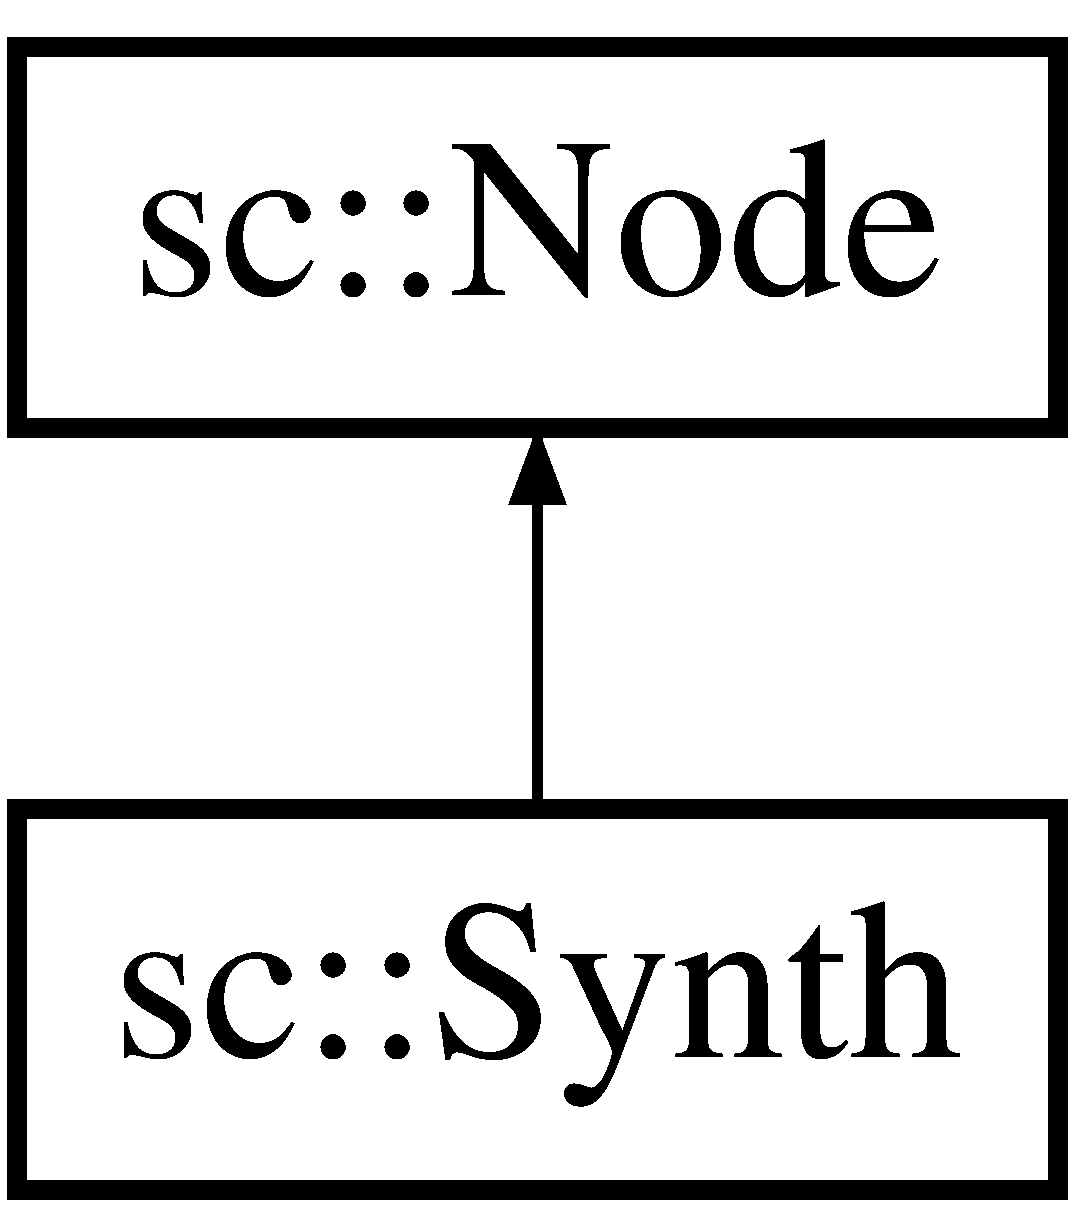
\includegraphics[height=2.000000cm]{classsc_1_1Synth}
\end{center}
\end{figure}
\subsection*{Public Member Functions}
\begin{DoxyCompactItemize}
\item 
\hyperlink{classsc_1_1Synth_ab3bf5c5976bd7c0bcbaa8cae4cb4be8d}{Synth} (\hyperlink{classsc_1_1SCServer}{S\-C\-Server} $\ast$other, const std\-::string \&def\-Name, int id\-\_\-, int init\-Action=0, int add\-Action=T\-O\-\_\-\-H\-E\-A\-D, int target=D\-E\-F\-A\-U\-L\-T\-\_\-\-G\-R\-O\-U\-P)
\item 
\hyperlink{classsc_1_1Synth_af48d7363fd76ffe704559705f5011328}{Synth} (\hyperlink{classsc_1_1SCServer}{S\-C\-Server} $\ast$other, const std\-::string \&def\-Name, int id\-\_\-, std\-::map$<$ std\-::string, float $>$ \&args, int init\-Action=0, int add\-Action=T\-O\-\_\-\-H\-E\-A\-D, int target=D\-E\-F\-A\-U\-L\-T\-\_\-\-G\-R\-O\-U\-P)
\item 
\hypertarget{classsc_1_1Synth_a1b52cbfb16f211e3d5ae909eed6420eb}{\hyperlink{classsc_1_1Synth_a1b52cbfb16f211e3d5ae909eed6420eb}{$\sim$\-Synth} ()}\label{classsc_1_1Synth_a1b52cbfb16f211e3d5ae909eed6420eb}

\begin{DoxyCompactList}\small\item\em Destructor. \end{DoxyCompactList}\end{DoxyCompactItemize}


\subsection{Detailed Description}
This class represents a client-\/side version of a server synth. 

\subsection{Constructor \& Destructor Documentation}
\hypertarget{classsc_1_1Synth_ab3bf5c5976bd7c0bcbaa8cae4cb4be8d}{\index{sc\-::\-Synth@{sc\-::\-Synth}!Synth@{Synth}}
\index{Synth@{Synth}!sc::Synth@{sc\-::\-Synth}}
\subsubsection[{Synth}]{\setlength{\rightskip}{0pt plus 5cm}sc\-::\-Synth\-::\-Synth (
\begin{DoxyParamCaption}
\item[{{\bf S\-C\-Server} $\ast$}]{other, }
\item[{const std\-::string \&}]{def\-Name, }
\item[{int}]{id\-\_\-, }
\item[{int}]{init\-Action = {\ttfamily 0}, }
\item[{int}]{add\-Action = {\ttfamily TO\-\_\-HEAD}, }
\item[{int}]{target = {\ttfamily DEFAULT\-\_\-GROUP}}
\end{DoxyParamCaption}
)}}\label{classsc_1_1Synth_ab3bf5c5976bd7c0bcbaa8cae4cb4be8d}
Create a \hyperlink{classsc_1_1Synth}{Synth} with a user defined name, id, add\-Action, and target If no add\-Action is specified, this \hyperlink{classsc_1_1Synth}{Synth} is added to the head of target group If no target group is specified, this \hyperlink{classsc_1_1Synth}{Synth} is added to the Default \hyperlink{classsc_1_1Group}{Group} 
\begin{DoxyParams}[1]{Parameters}
\mbox{\tt in}  & {\em S\-C\-Server\&} & \hyperlink{classsc_1_1SCServer}{S\-C\-Server} instance \\
\hline
\mbox{\tt in}  & {\em const} & std\-::string\& def\-Name \\
\hline
\mbox{\tt in}  & {\em int} & Id \\
\hline
\mbox{\tt in}  & {\em int} & Add Action \\
\hline
\mbox{\tt in}  & {\em int} & Target \hyperlink{classsc_1_1Group}{Group} \\
\hline
\end{DoxyParams}
\hypertarget{classsc_1_1Synth_af48d7363fd76ffe704559705f5011328}{\index{sc\-::\-Synth@{sc\-::\-Synth}!Synth@{Synth}}
\index{Synth@{Synth}!sc::Synth@{sc\-::\-Synth}}
\subsubsection[{Synth}]{\setlength{\rightskip}{0pt plus 5cm}sc\-::\-Synth\-::\-Synth (
\begin{DoxyParamCaption}
\item[{{\bf S\-C\-Server} $\ast$}]{other, }
\item[{const std\-::string \&}]{def\-Name, }
\item[{int}]{id\-\_\-, }
\item[{std\-::map$<$ std\-::string, float $>$ \&}]{args, }
\item[{int}]{init\-Action = {\ttfamily 0}, }
\item[{int}]{add\-Action = {\ttfamily TO\-\_\-HEAD}, }
\item[{int}]{target = {\ttfamily DEFAULT\-\_\-GROUP}}
\end{DoxyParamCaption}
)}}\label{classsc_1_1Synth_af48d7363fd76ffe704559705f5011328}
Create a \hyperlink{classsc_1_1Synth}{Synth} with a user defined name, id, \hyperlink{classsc_1_1Node}{Node} args, add\-Action, and target If no add\-Action is specified, this \hyperlink{classsc_1_1Synth}{Synth} is added to the head of target group If no target group is specified, this \hyperlink{classsc_1_1Synth}{Synth} is added to the Default \hyperlink{classsc_1_1Group}{Group} 
\begin{DoxyParams}[1]{Parameters}
\mbox{\tt in}  & {\em S\-C\-Server\&} & \hyperlink{classsc_1_1SCServer}{S\-C\-Server} instance \\
\hline
\mbox{\tt in}  & {\em const} & std\-::string\& def\-Name \\
\hline
\mbox{\tt in}  & {\em int} & Id \\
\hline
\mbox{\tt in}  & {\em std\-::map$<$std\-::string,float$>$} & Args \\
\hline
\mbox{\tt in}  & {\em int} & Add Action \\
\hline
\mbox{\tt in}  & {\em int} & Target \hyperlink{classsc_1_1Group}{Group} \\
\hline
\end{DoxyParams}


The documentation for this class was generated from the following file\-:\begin{DoxyCompactItemize}
\item 
include/\hyperlink{Node_8hpp}{Node.\-hpp}\end{DoxyCompactItemize}

\chapter{File Documentation}
\hypertarget{Buffer_8hpp}{\section{include/\-Buffer.hpp File Reference}
\label{Buffer_8hpp}\index{include/\-Buffer.\-hpp@{include/\-Buffer.\-hpp}}
}


Header file for \hyperlink{Buffer_8hpp}{Buffer.\-hpp}.  


{\ttfamily \#include \char`\"{}S\-C\-Server.\-hpp\char`\"{}}\\*
\subsection*{Classes}
\begin{DoxyCompactItemize}
\item 
class \hyperlink{classsc_1_1Buffer}{sc\-::\-Buffer}
\begin{DoxyCompactList}\small\item\em This class represents a client-\/side version of a server buffer. \end{DoxyCompactList}\end{DoxyCompactItemize}


\subsection{Detailed Description}
Header file for \hyperlink{Buffer_8hpp}{Buffer.\-hpp}. \begin{DoxyAuthor}{Author}
Eric Hamdan \href{mailto:erichamdan@gmail.com}{\tt erichamdan@gmail.\-com} 
\end{DoxyAuthor}

\hypertarget{Bus_8hpp}{\section{include/\-Bus.hpp File Reference}
\label{Bus_8hpp}\index{include/\-Bus.\-hpp@{include/\-Bus.\-hpp}}
}


Header file for \hyperlink{Bus_8hpp}{Bus.\-hpp}.  


{\ttfamily \#include $<$vector$>$}\\*
\subsection*{Classes}
\begin{DoxyCompactItemize}
\item 
class \hyperlink{classColliderPlusPlus_1_1Bus}{Collider\-Plus\-Plus\-::\-Bus}
\begin{DoxyCompactList}\small\item\em This class represents a client-\/side version of a server bus. \end{DoxyCompactList}\end{DoxyCompactItemize}


\subsection{Detailed Description}
Header file for \hyperlink{Bus_8hpp}{Bus.\-hpp}. \begin{DoxyAuthor}{Author}
Eric Hamdan \href{mailto:erichamdan@gmail.com}{\tt erichamdan@gmail.\-com} 
\end{DoxyAuthor}

\hypertarget{Node_8hpp}{\section{include/\-Node.hpp File Reference}
\label{Node_8hpp}\index{include/\-Node.\-hpp@{include/\-Node.\-hpp}}
}


Header file for \hyperlink{Node_8hpp}{Node.\-hpp}.  


{\ttfamily \#include \char`\"{}S\-C\-Server.\-hpp\char`\"{}}\\*
{\ttfamily \#include \char`\"{}Bus.\-hpp\char`\"{}}\\*
{\ttfamily \#include $<$string$>$}\\*
{\ttfamily \#include $<$map$>$}\\*
\subsection*{Classes}
\begin{DoxyCompactItemize}
\item 
class \hyperlink{classsc_1_1Node}{sc\-::\-Node}
\begin{DoxyCompactList}\small\item\em This class represents a client-\/side version of a server node (\hyperlink{classsc_1_1Synth}{Synth} or \hyperlink{classsc_1_1Group}{Group}) \end{DoxyCompactList}\item 
class \hyperlink{classsc_1_1Synth}{sc\-::\-Synth}
\begin{DoxyCompactList}\small\item\em This class represents a client-\/side version of a server synth. \end{DoxyCompactList}\item 
class \hyperlink{classsc_1_1Group}{sc\-::\-Group}
\begin{DoxyCompactList}\small\item\em This class represents a client-\/side version of a server group. \end{DoxyCompactList}\item 
class \hyperlink{classsc_1_1RootNode}{sc\-::\-Root\-Node}
\begin{DoxyCompactList}\small\item\em This class represents a client-\/side version of a server root node. \end{DoxyCompactList}\end{DoxyCompactItemize}


\subsection{Detailed Description}
Header file for \hyperlink{Node_8hpp}{Node.\-hpp}. \begin{DoxyAuthor}{Author}
Eric Hamdan \href{mailto:erichamdan@gmail.com}{\tt erichamdan@gmail.\-com} 
\end{DoxyAuthor}

\hypertarget{SCServer_8hpp}{\section{include/\-S\-C\-Server.hpp File Reference}
\label{SCServer_8hpp}\index{include/\-S\-C\-Server.\-hpp@{include/\-S\-C\-Server.\-hpp}}
}


Header file for \hyperlink{SCServer_8hpp}{S\-C\-Server.\-hpp}.  


{\ttfamily \#include $<$string$>$}\\*
{\ttfamily \#include $<$vector$>$}\\*
{\ttfamily \#include $<$map$>$}\\*
{\ttfamily \#include \char`\"{}tny\-\_\-osc/tnyosc-\/dispatch.\-hpp\char`\"{}}\\*
{\ttfamily \#include \char`\"{}tny\-\_\-osc/tnyosc.\-hpp\char`\"{}}\\*
\subsection*{Classes}
\begin{DoxyCompactItemize}
\item 
class \hyperlink{classsc_1_1SCServer}{sc\-::\-S\-C\-Server}
\begin{DoxyCompactList}\small\item\em This class represents a client-\/side version of scsynth, the Super\-Collider audio server. \end{DoxyCompactList}\end{DoxyCompactItemize}
\subsection*{Macros}
\begin{DoxyCompactItemize}
\item 
\hypertarget{SCServer_8hpp_aec2817847ec8c92eb99257101ddf102d}{\#define {\bfseries T\-O\-\_\-\-H\-E\-A\-D}~0}\label{SCServer_8hpp_aec2817847ec8c92eb99257101ddf102d}

\item 
\hypertarget{SCServer_8hpp_a1347de071d12a2e8a25f51b2cc7d6808}{\#define {\bfseries T\-O\-\_\-\-T\-A\-I\-L}~1}\label{SCServer_8hpp_a1347de071d12a2e8a25f51b2cc7d6808}

\item 
\hypertarget{SCServer_8hpp_a59b85f0c6cd4fecb4b22fc304b3f987b}{\#define {\bfseries J\-U\-S\-T\-\_\-\-B\-E\-F\-O\-R\-E}~2}\label{SCServer_8hpp_a59b85f0c6cd4fecb4b22fc304b3f987b}

\item 
\hypertarget{SCServer_8hpp_aa87ca6e73fcb856bf2e1eb352456337d}{\#define {\bfseries J\-U\-S\-T\-\_\-\-A\-F\-T\-E\-R}~3}\label{SCServer_8hpp_aa87ca6e73fcb856bf2e1eb352456337d}

\item 
\hypertarget{SCServer_8hpp_ac5e6ea3bc12db0b69fd25d64090fcb93}{\#define {\bfseries R\-E\-P\-L\-A\-C\-E}~4}\label{SCServer_8hpp_ac5e6ea3bc12db0b69fd25d64090fcb93}

\item 
\hypertarget{SCServer_8hpp_a13ee4e75a35c2ef819d4bff181d6bae3}{\#define {\bfseries R\-O\-O\-T\-\_\-\-N\-O\-D\-E}~0}\label{SCServer_8hpp_a13ee4e75a35c2ef819d4bff181d6bae3}

\item 
\hypertarget{SCServer_8hpp_a45b6308e1477048e29afac209cfe9ec1}{\#define {\bfseries D\-E\-F\-A\-U\-L\-T\-\_\-\-G\-R\-O\-U\-P}~1}\label{SCServer_8hpp_a45b6308e1477048e29afac209cfe9ec1}

\item 
\hypertarget{SCServer_8hpp_a47d6a9f1bcd63b2386f7174e14f86345}{\#define {\bfseries S\-Y\-N\-T\-H}~1}\label{SCServer_8hpp_a47d6a9f1bcd63b2386f7174e14f86345}

\item 
\hypertarget{SCServer_8hpp_a5f6b617b45eb12646bb651ecf77f6dcd}{\#define {\bfseries G\-R\-O\-U\-P}~2}\label{SCServer_8hpp_a5f6b617b45eb12646bb651ecf77f6dcd}

\end{DoxyCompactItemize}


\subsection{Detailed Description}
Header file for \hyperlink{SCServer_8hpp}{S\-C\-Server.\-hpp}. \begin{DoxyAuthor}{Author}
Eric Hamdan \href{mailto:erichamdan@gmail.com}{\tt erichamdan@gmail.\-com} 
\end{DoxyAuthor}

\hypertarget{Sound_8hpp}{\section{include/\-Sound.hpp File Reference}
\label{Sound_8hpp}\index{include/\-Sound.\-hpp@{include/\-Sound.\-hpp}}
}


Header file for \hyperlink{Sound_8hpp}{Sound.\-hpp}.  


{\ttfamily \#include $<$string$>$}\\*
{\ttfamily \#include $<$map$>$}\\*
{\ttfamily \#include \char`\"{}Buffer.\-hpp\char`\"{}}\\*
{\ttfamily \#include \char`\"{}S\-C\-Server.\-hpp\char`\"{}}\\*
{\ttfamily \#include \char`\"{}Node.\-hpp\char`\"{}}\\*
\subsection*{Classes}
\begin{DoxyCompactItemize}
\item 
class \hyperlink{classsc_1_1Sound}{sc\-::\-Sound}
\begin{DoxyCompactList}\small\item\em This class represents a user manipulable Soundfile Player, essentially mirroring the O\-A\-S class of the same name by Shreenidhi Chowkwale  \href{https://github.com/CalVR/Open-Audio-Server/blob/master/client/src/Sound.h}{\tt https\-://github.\-com/\-Cal\-V\-R/\-Open-\/\-Audio-\/\-Server/blob/master/client/src/\-Sound.\-h}. \end{DoxyCompactList}\end{DoxyCompactItemize}
\subsection*{Macros}
\begin{DoxyCompactItemize}
\item 
\hypertarget{Sound_8hpp_a13c6b09218723edb5010bcfa833a23b5}{\#define {\bfseries N\-E\-W\-\_\-\-P\-A\-U\-S\-E\-D}~0}\label{Sound_8hpp_a13c6b09218723edb5010bcfa833a23b5}

\item 
\hypertarget{Sound_8hpp_ab6bca16ed021b1e211fde8669758f199}{\#define {\bfseries N\-E\-W}~1}\label{Sound_8hpp_ab6bca16ed021b1e211fde8669758f199}

\end{DoxyCompactItemize}


\subsection{Detailed Description}
Header file for \hyperlink{Sound_8hpp}{Sound.\-hpp}. \begin{DoxyAuthor}{Author}
Eric Hamdan \href{mailto:erichamdan@gmail.com}{\tt erichamdan@gmail.\-com} 
\end{DoxyAuthor}

\addcontentsline{toc}{part}{Index}
\printindex
\end{document}
